\chapter{Increment 2 Screenshots}

\begin{figure}[!ht]
    \centering
    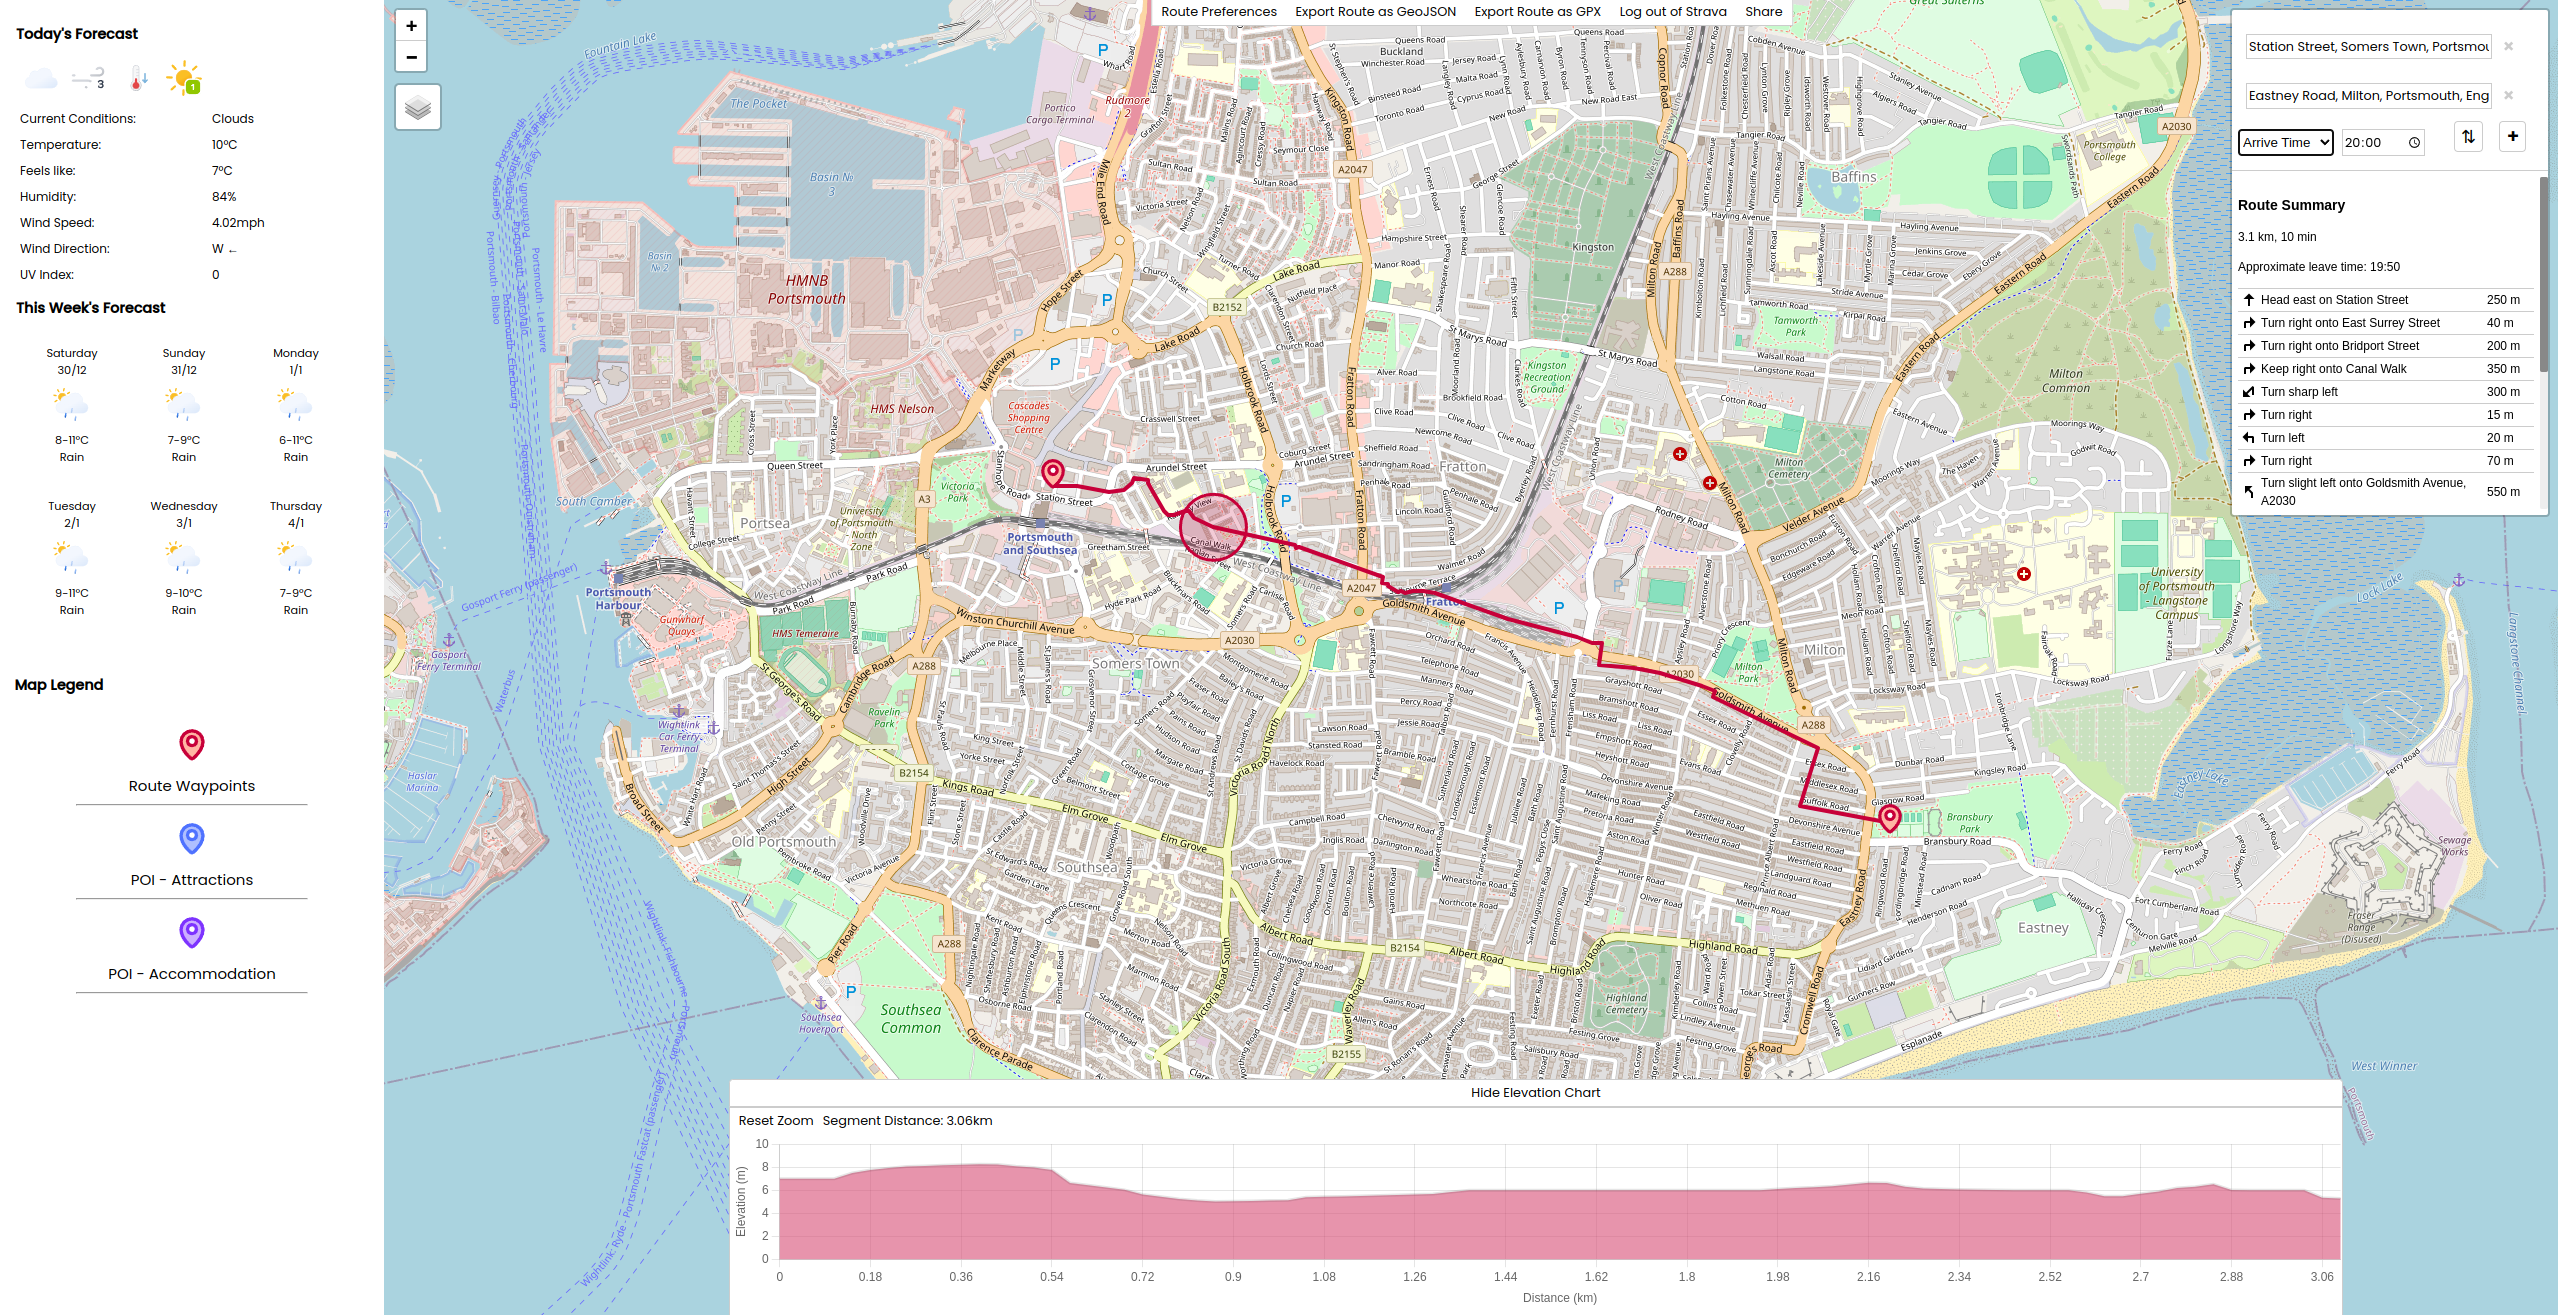
\includegraphics[width=425px]{figures/Progress Images/Iteration-2/SR9-10/SR9 - Arrive Time.png}
    \caption{Arrive Time Implementation}
    \label{fig:arrive-time}
\end{figure}

\begin{figure}[!ht]
    \centering
    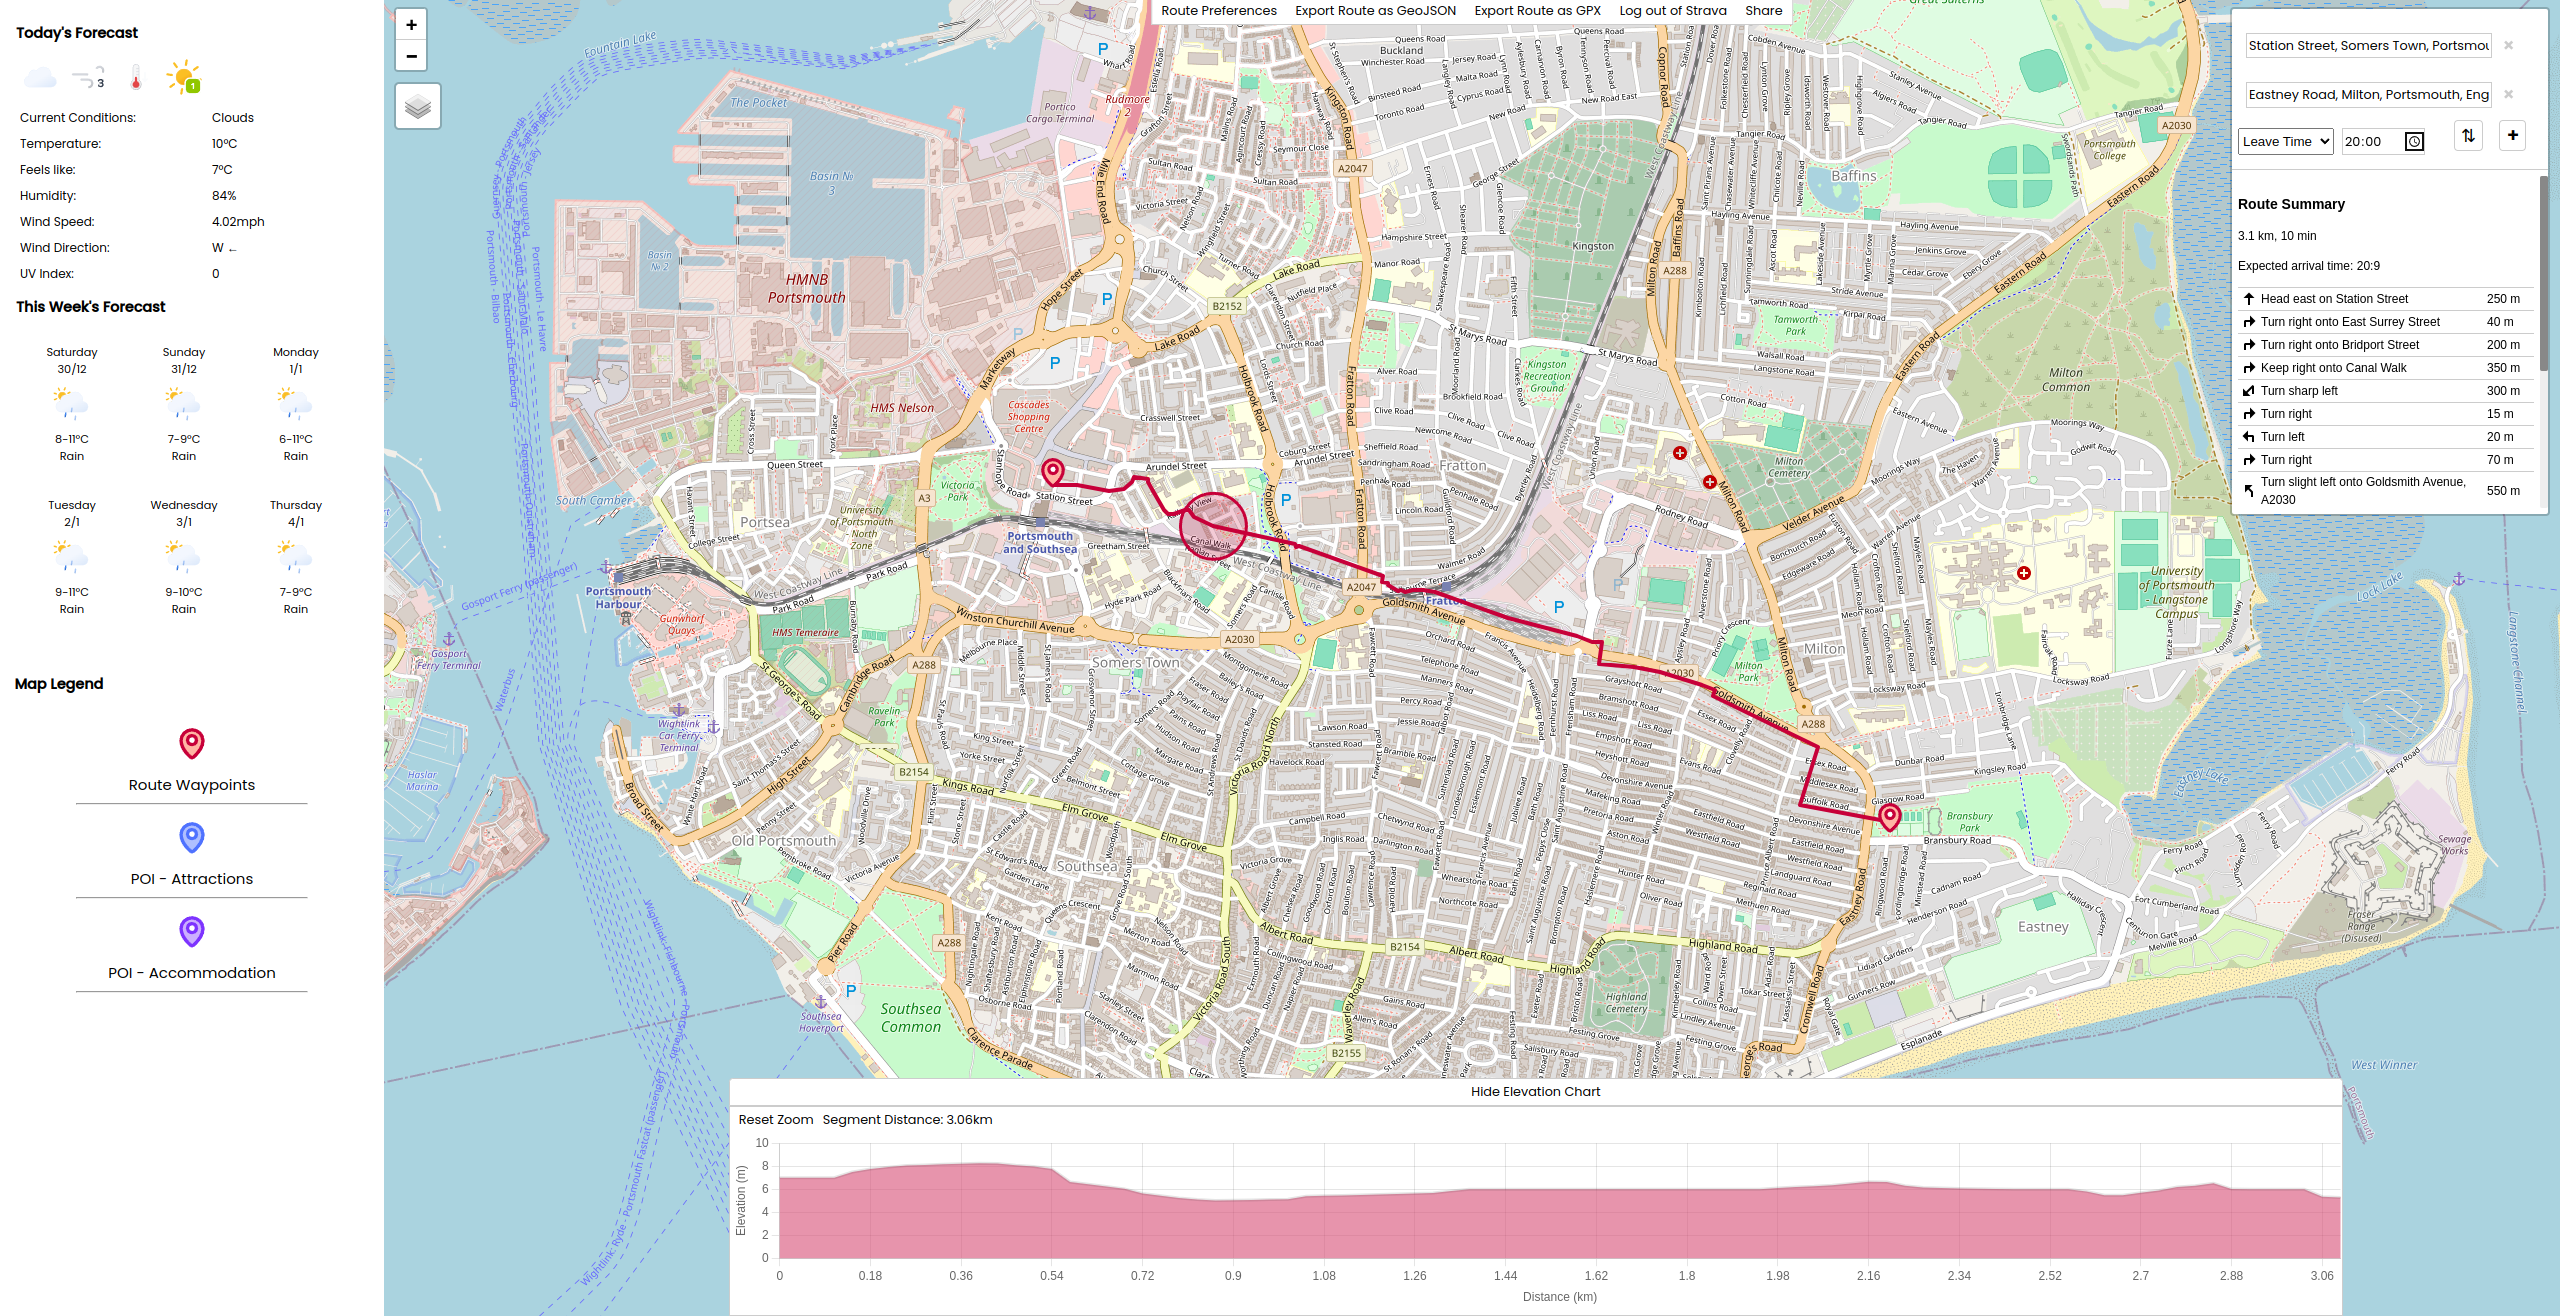
\includegraphics[width=425px]{figures/Progress Images/Iteration-2/SR9-10/SR9 - Leave Time.png}
    \caption{Leave Time Implementation}
    \label{fig:leave-time}
\end{figure}

\begin{figure}[!ht]
    \centering
    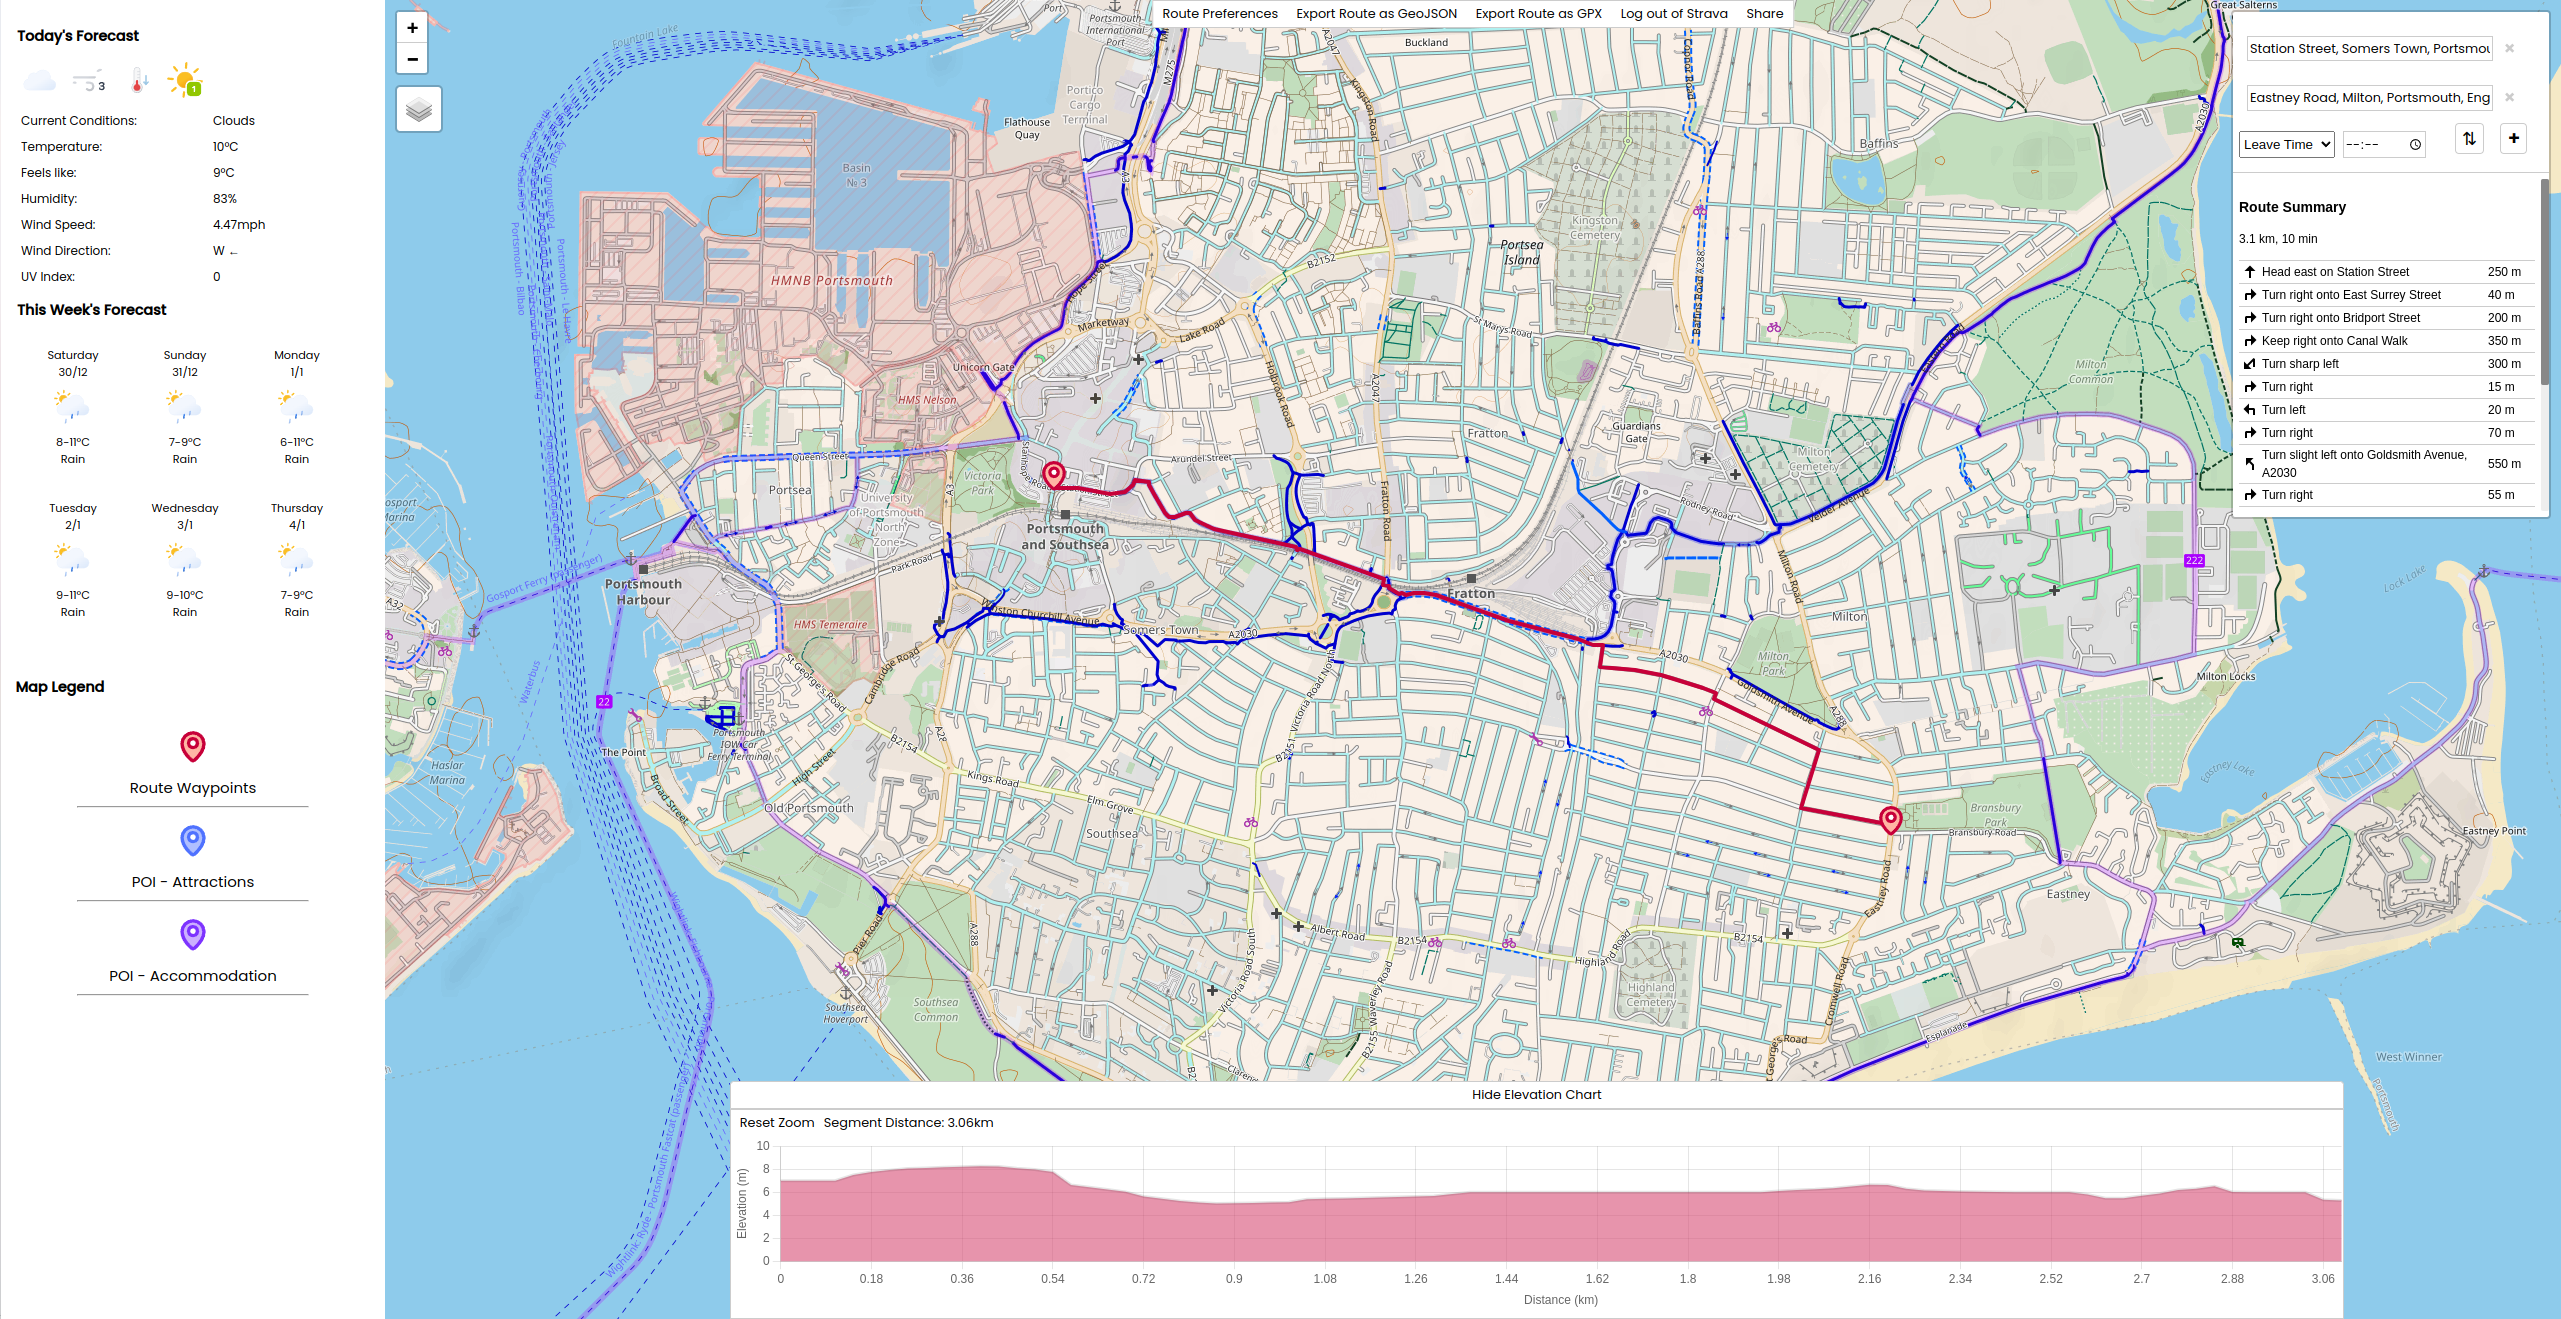
\includegraphics[width=425px]{figures/Progress Images/Iteration-2/SR9-10/SR9_10 - Leave_Arrival Time.png}
    \caption{Arrive/Leave Time Final}
    \label{fig:arrive-leave-time}
\end{figure}

\begin{figure}[!ht]
    \centering
    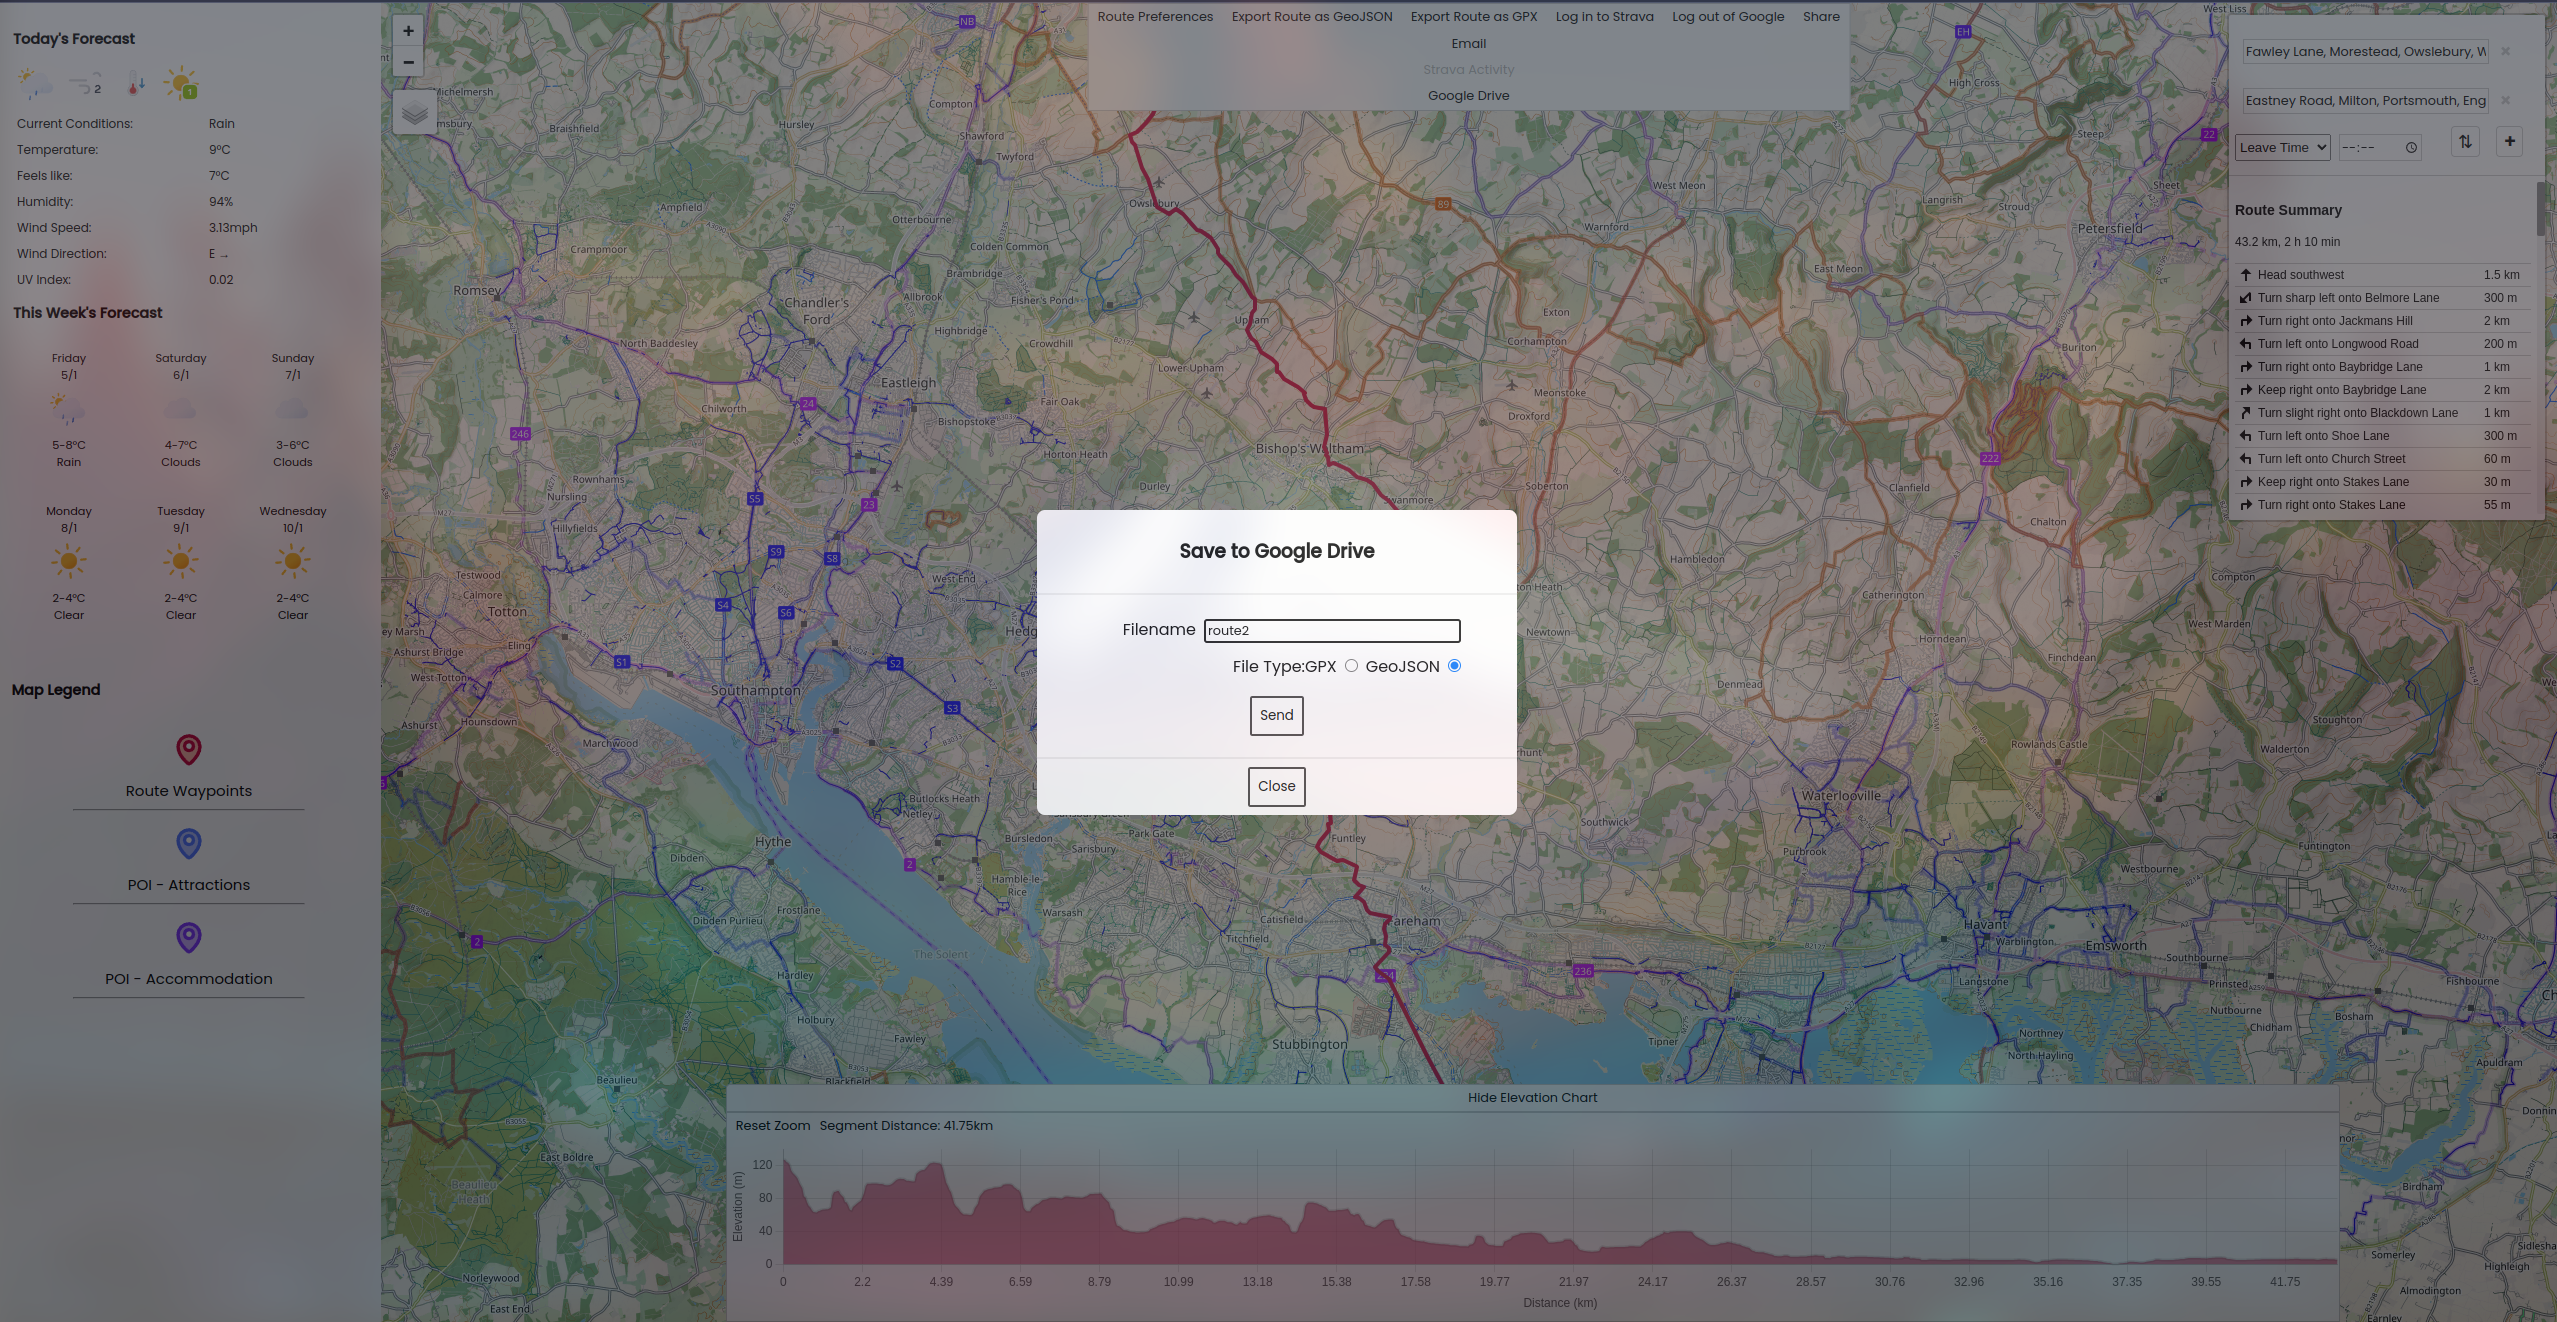
\includegraphics[width=425px]{figures/Progress Images/Iteration-2/SR15/SR15 - Save to GDrive Modal working.png}
    \caption{Google Drive Implementation}
    \label{fig:gdrive}
\end{figure}

\begin{figure}[!ht]
    \centering
    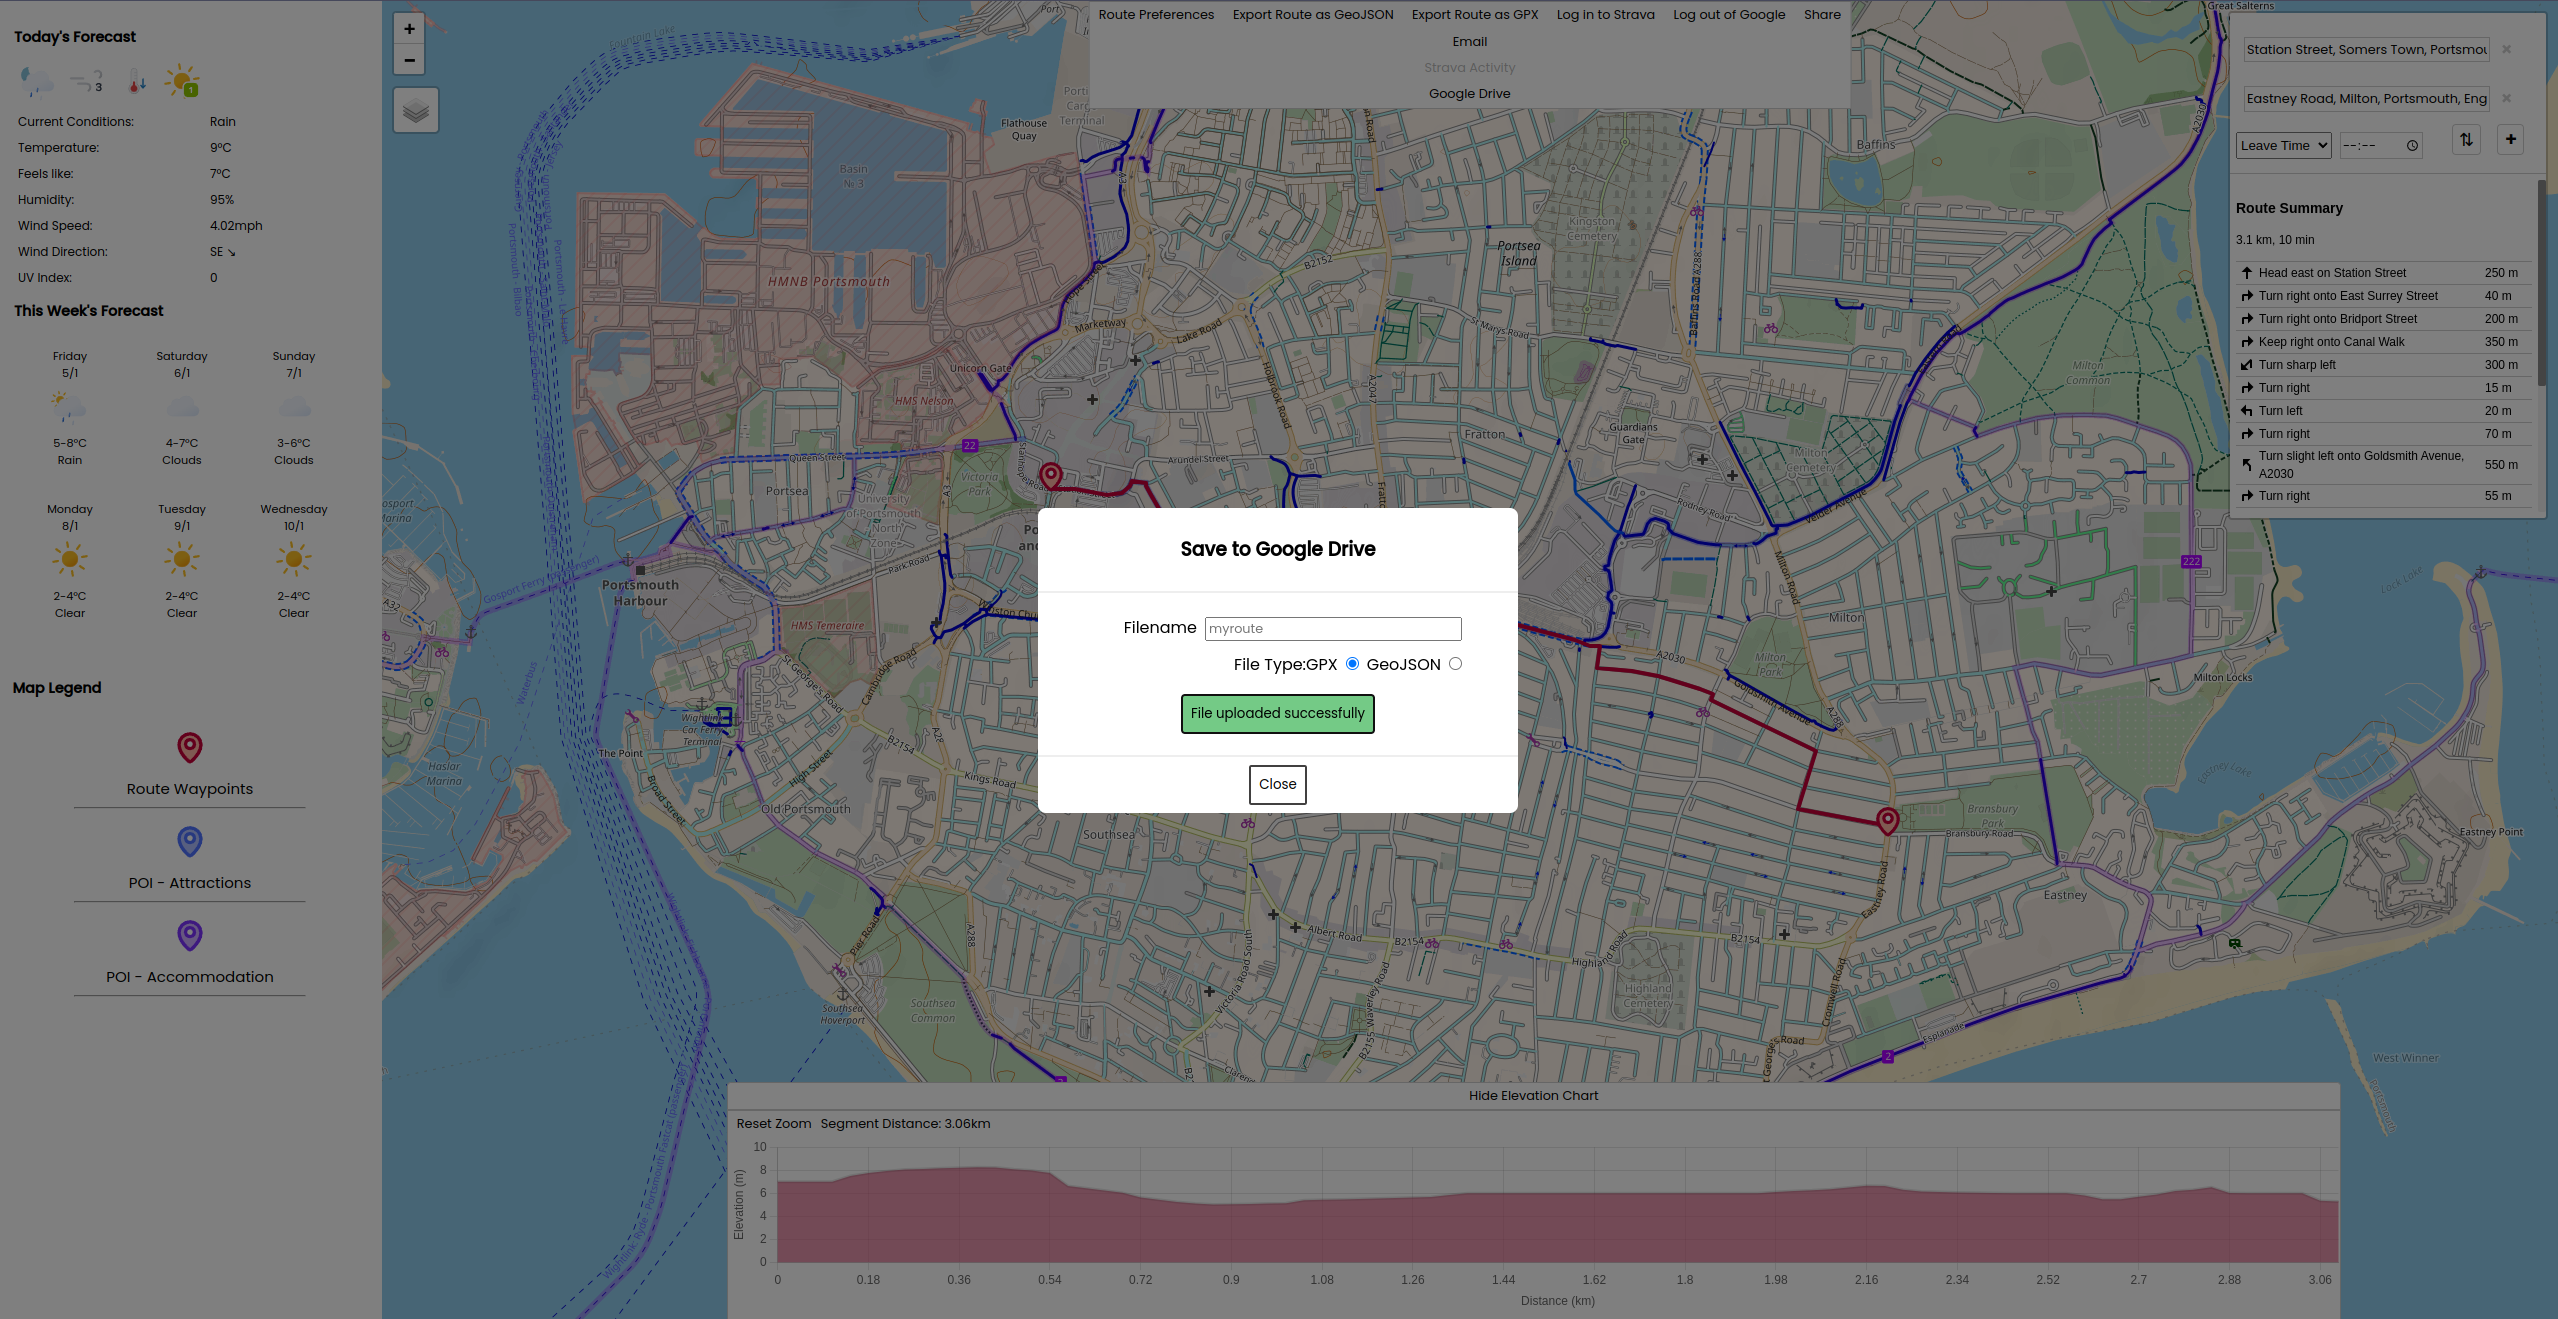
\includegraphics[width=425px]{figures/Progress Images/Iteration-2/SR15/SR15 - Success.png}
    \caption{Google Drive Implementation Success}
    \label{fig:gdrive-success}
\end{figure}

\begin{figure}[!ht]
    \centering
    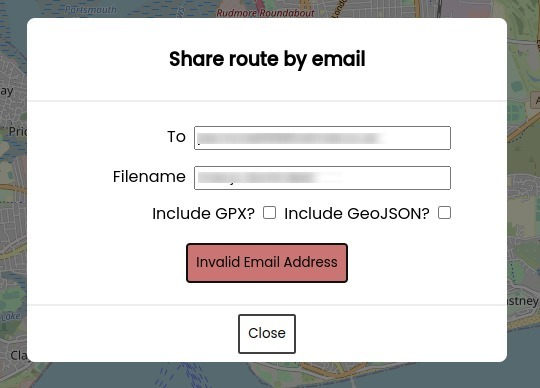
\includegraphics[width=425px]{figures/Progress Images/Iteration-2/SR17/SR17 Invalid Email.png}
    \caption{Invalid Email}
    \label{fig:invalid-email}
\end{figure}

\begin{figure}[!ht]
    \centering
    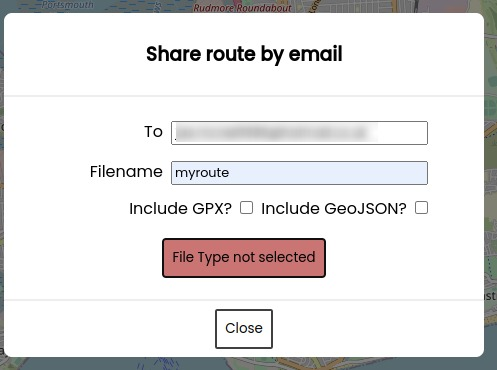
\includegraphics[width=425px]{figures/Progress Images/Iteration-2/SR17/SR17 Invalid File type.png}
    \caption{Invalid File Type}
    \label{fig:invalid-file}
\end{figure}

\begin{figure}[!ht]
    \centering
    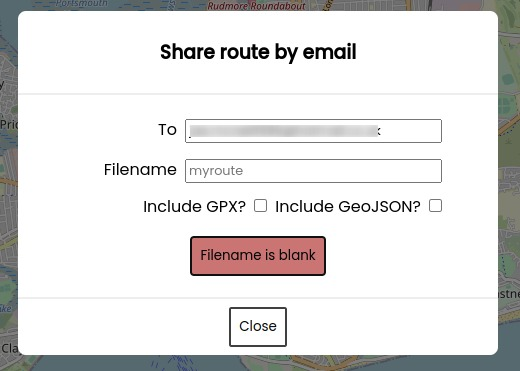
\includegraphics[width=425px]{figures/Progress Images/Iteration-2/SR17/SR17 Invalid Filename.png}
    \caption{Invalid Filename}
    \label{fig:invalid-filename}
\end{figure}

\begin{figure}[!ht]
    \centering
    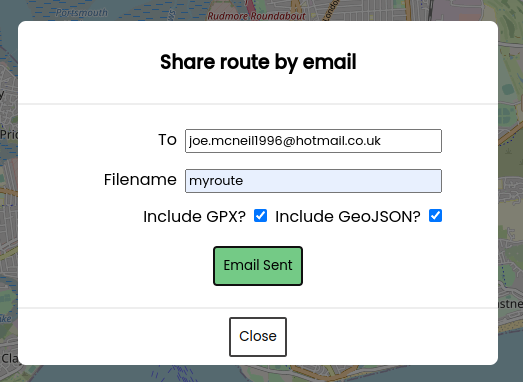
\includegraphics[width=425px]{figures/Progress Images/Iteration-2/SR17/SR17 Success.png}
    \caption{Email Success}
    \label{fig:email-success}
\end{figure}

\begin{figure}[!ht]
    \centering
    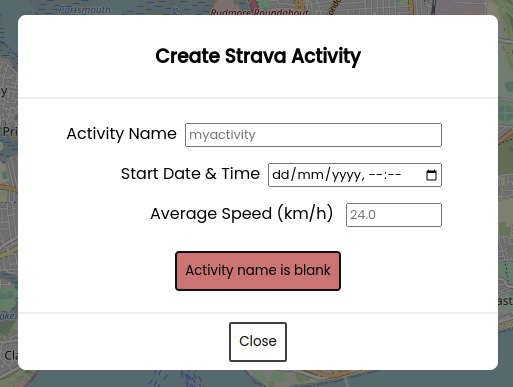
\includegraphics[width=425px]{figures/Progress Images/Iteration-2/SR18/SR18 Create Activity Fail - Missing Activity Name.png}
    \caption{Strava Missing Activity Name}
    \label{fig:missing-activity-name-strava}
\end{figure}

\begin{figure}[!ht]
    \centering
    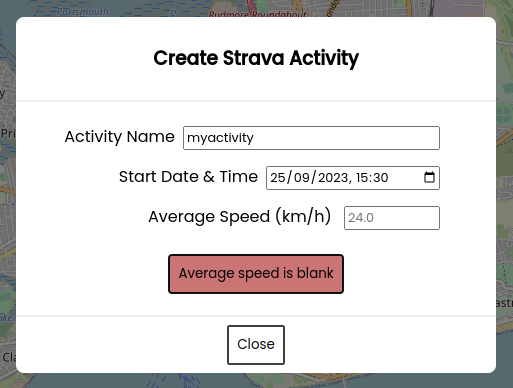
\includegraphics[width=425px]{figures/Progress Images/Iteration-2/SR18/SR18 Create Activity Fail - Missing Avg Speed.png}
    \caption{strava Missing Speed}
    \label{fig:missing-activity-speed-strava}
\end{figure}

\begin{figure}[!ht]
    \centering
    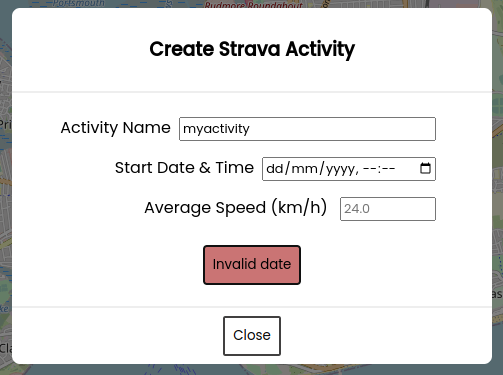
\includegraphics[width=425px]{figures/Progress Images/Iteration-2/SR18/SR18 Create Activity Fail - Missing DateTime.png}
    \caption{Strava Missing Date}
    \label{fig:missing-date-strava}
\end{figure}

\begin{figure}[!ht]
    \centering
    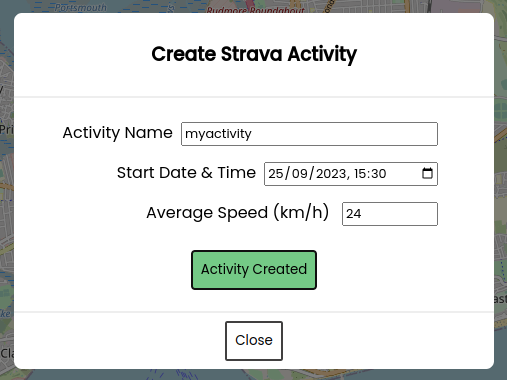
\includegraphics[width=425px]{figures/Progress Images/Iteration-2/SR18/SR18 Create Activity Success.png}
    \caption{Strava Activity Success}
    \label{fig:success-strava}
\end{figure}

\begin{figure}[!ht]
    \centering
    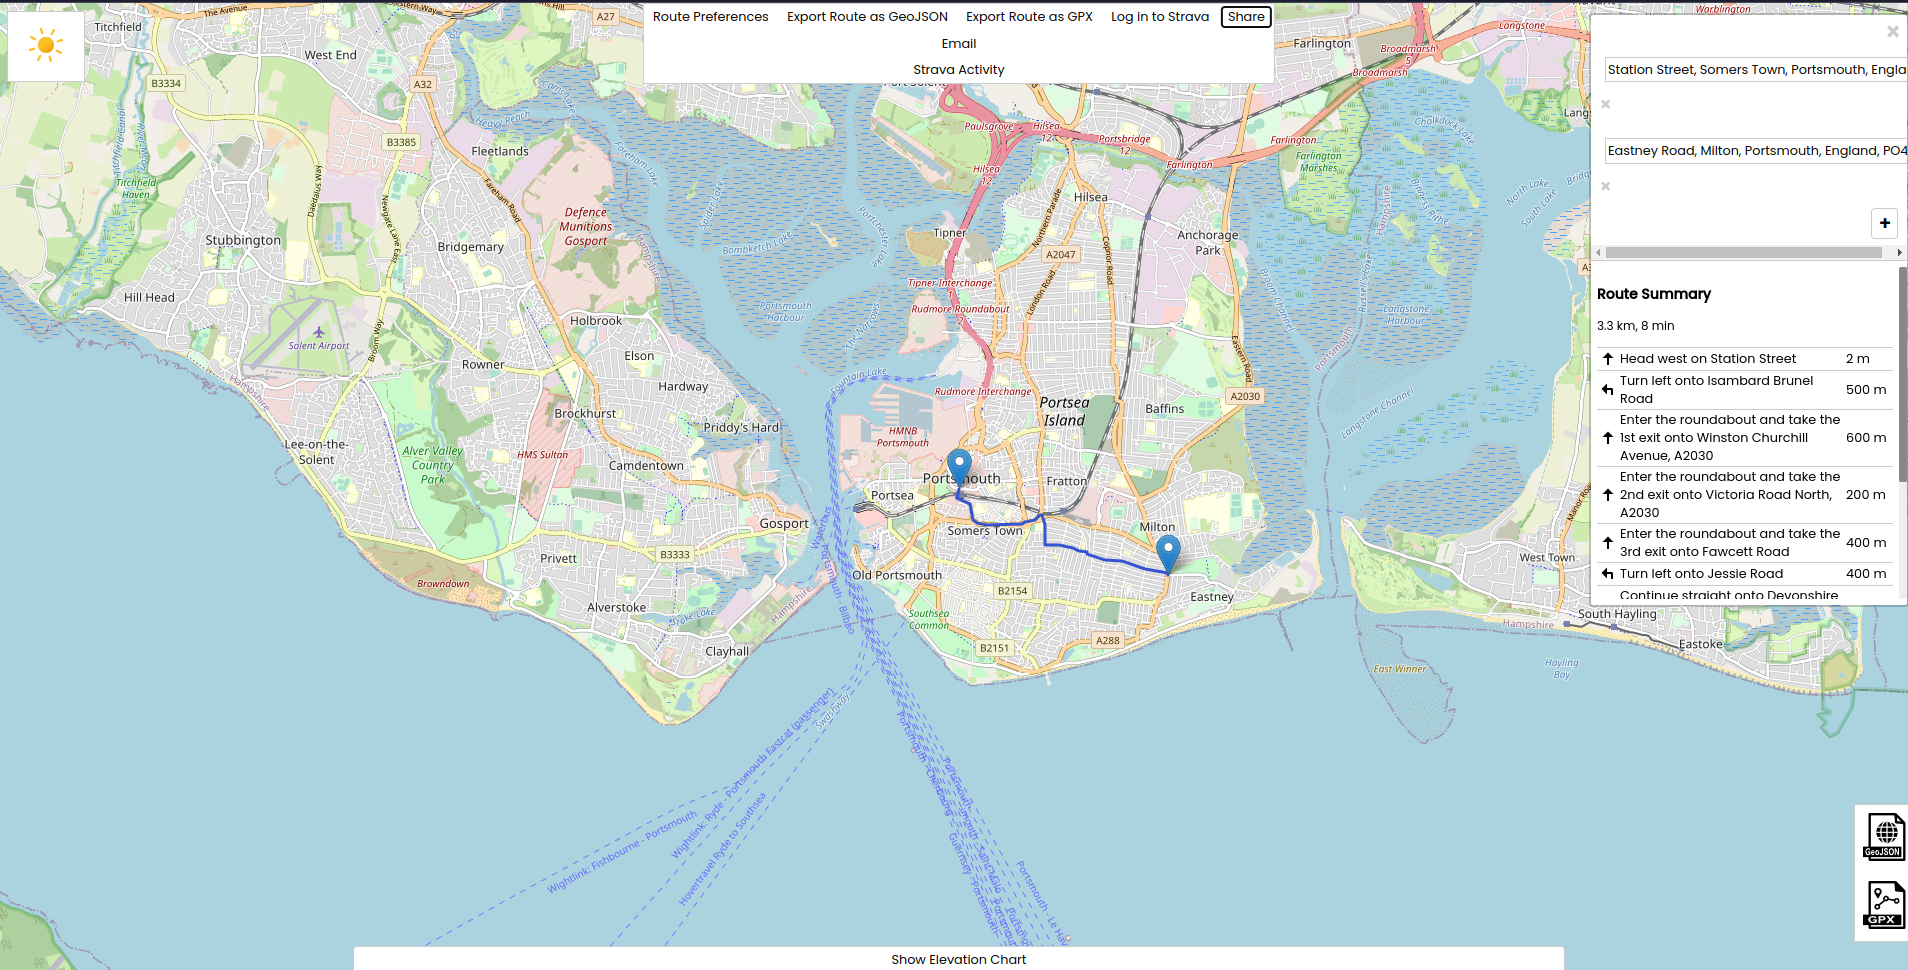
\includegraphics[width=425px]{figures/Progress Images/Iteration-2/SR18/SR18 Share Panel.png}
    \caption{Share Panel}
    \label{fig:share}
\end{figure}

\begin{figure}[!ht]
    \centering
    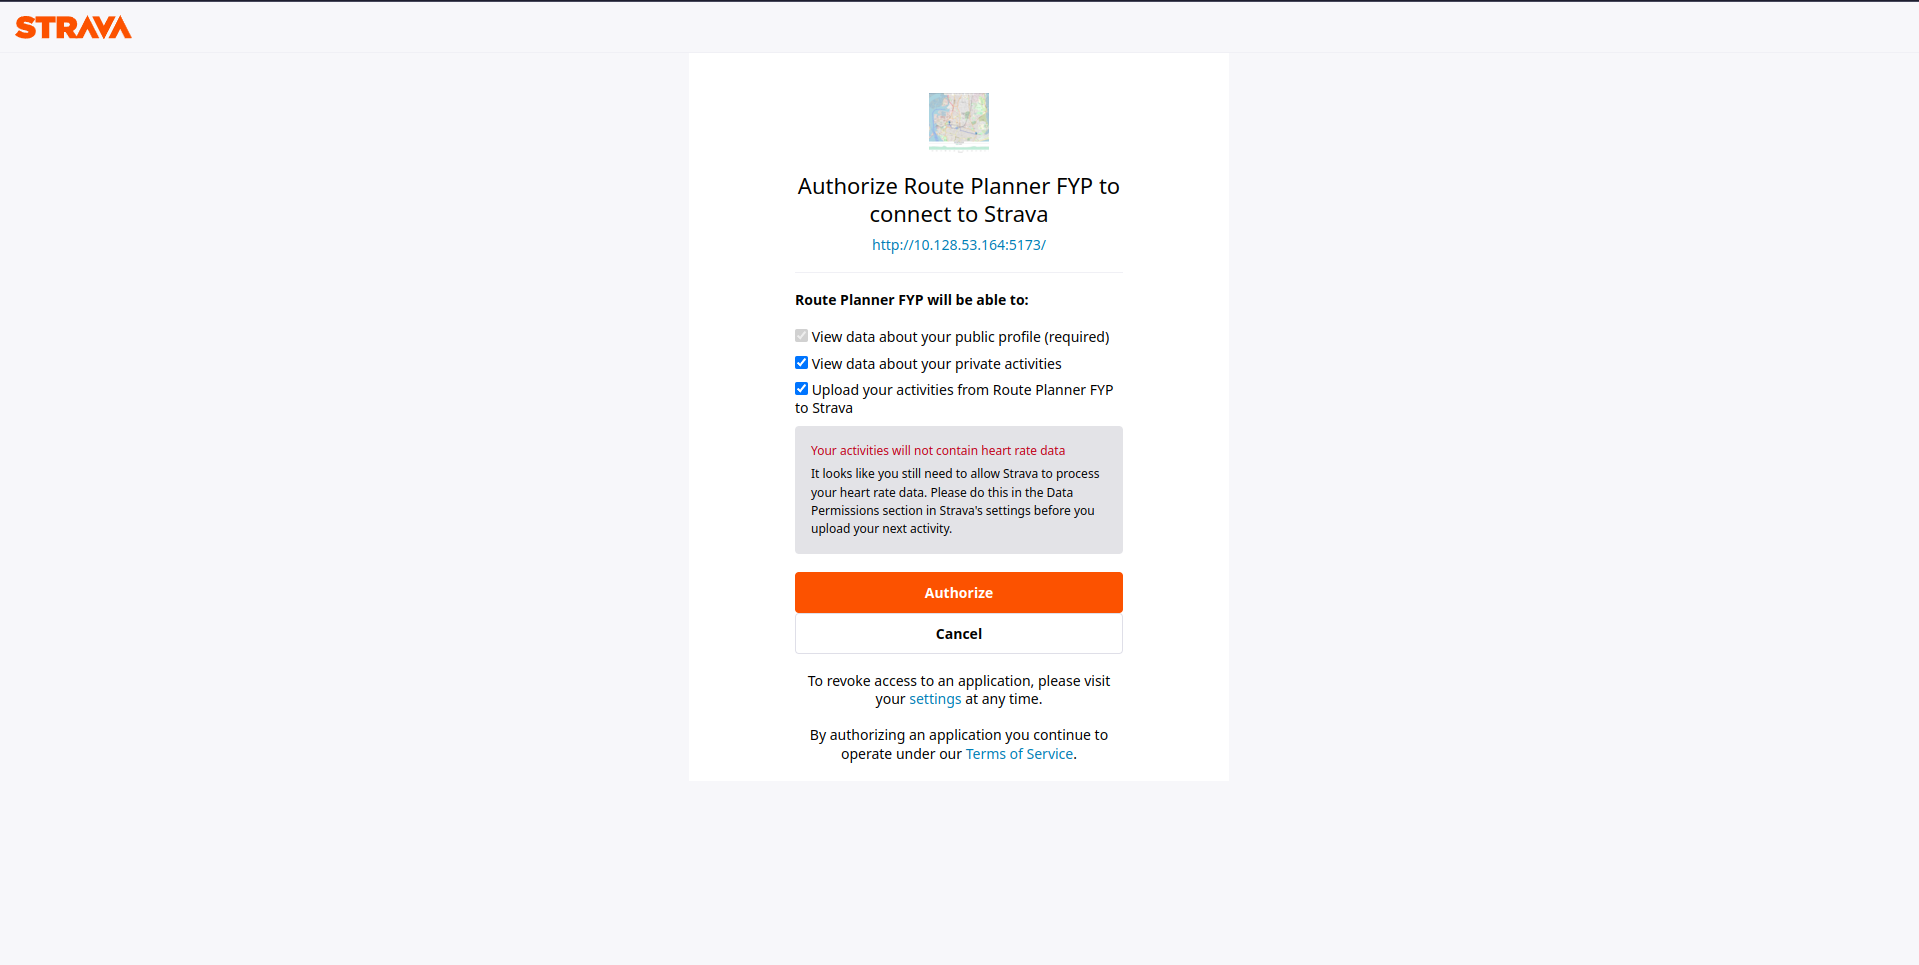
\includegraphics[width=425px]{figures/Progress Images/Iteration-2/SR18/SR18 Strava Auth.png}
    \caption{Strava Auth}
    \label{fig:auth-strava}
\end{figure}

\begin{figure}[!ht]
    \centering
    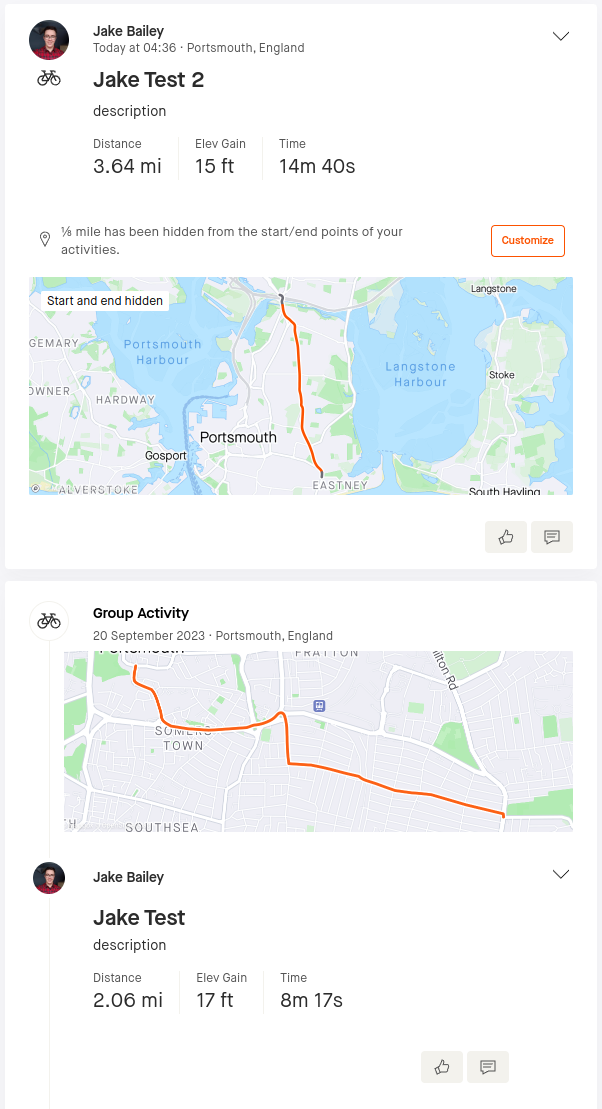
\includegraphics[width=300px]{figures/Progress Images/Iteration-2/SR18/SR18 Strava Example 3.png}
    \caption{Strava Example Upload}
    \label{fig:upload-strava}
\end{figure}

\begin{figure}[!ht]
    \centering
    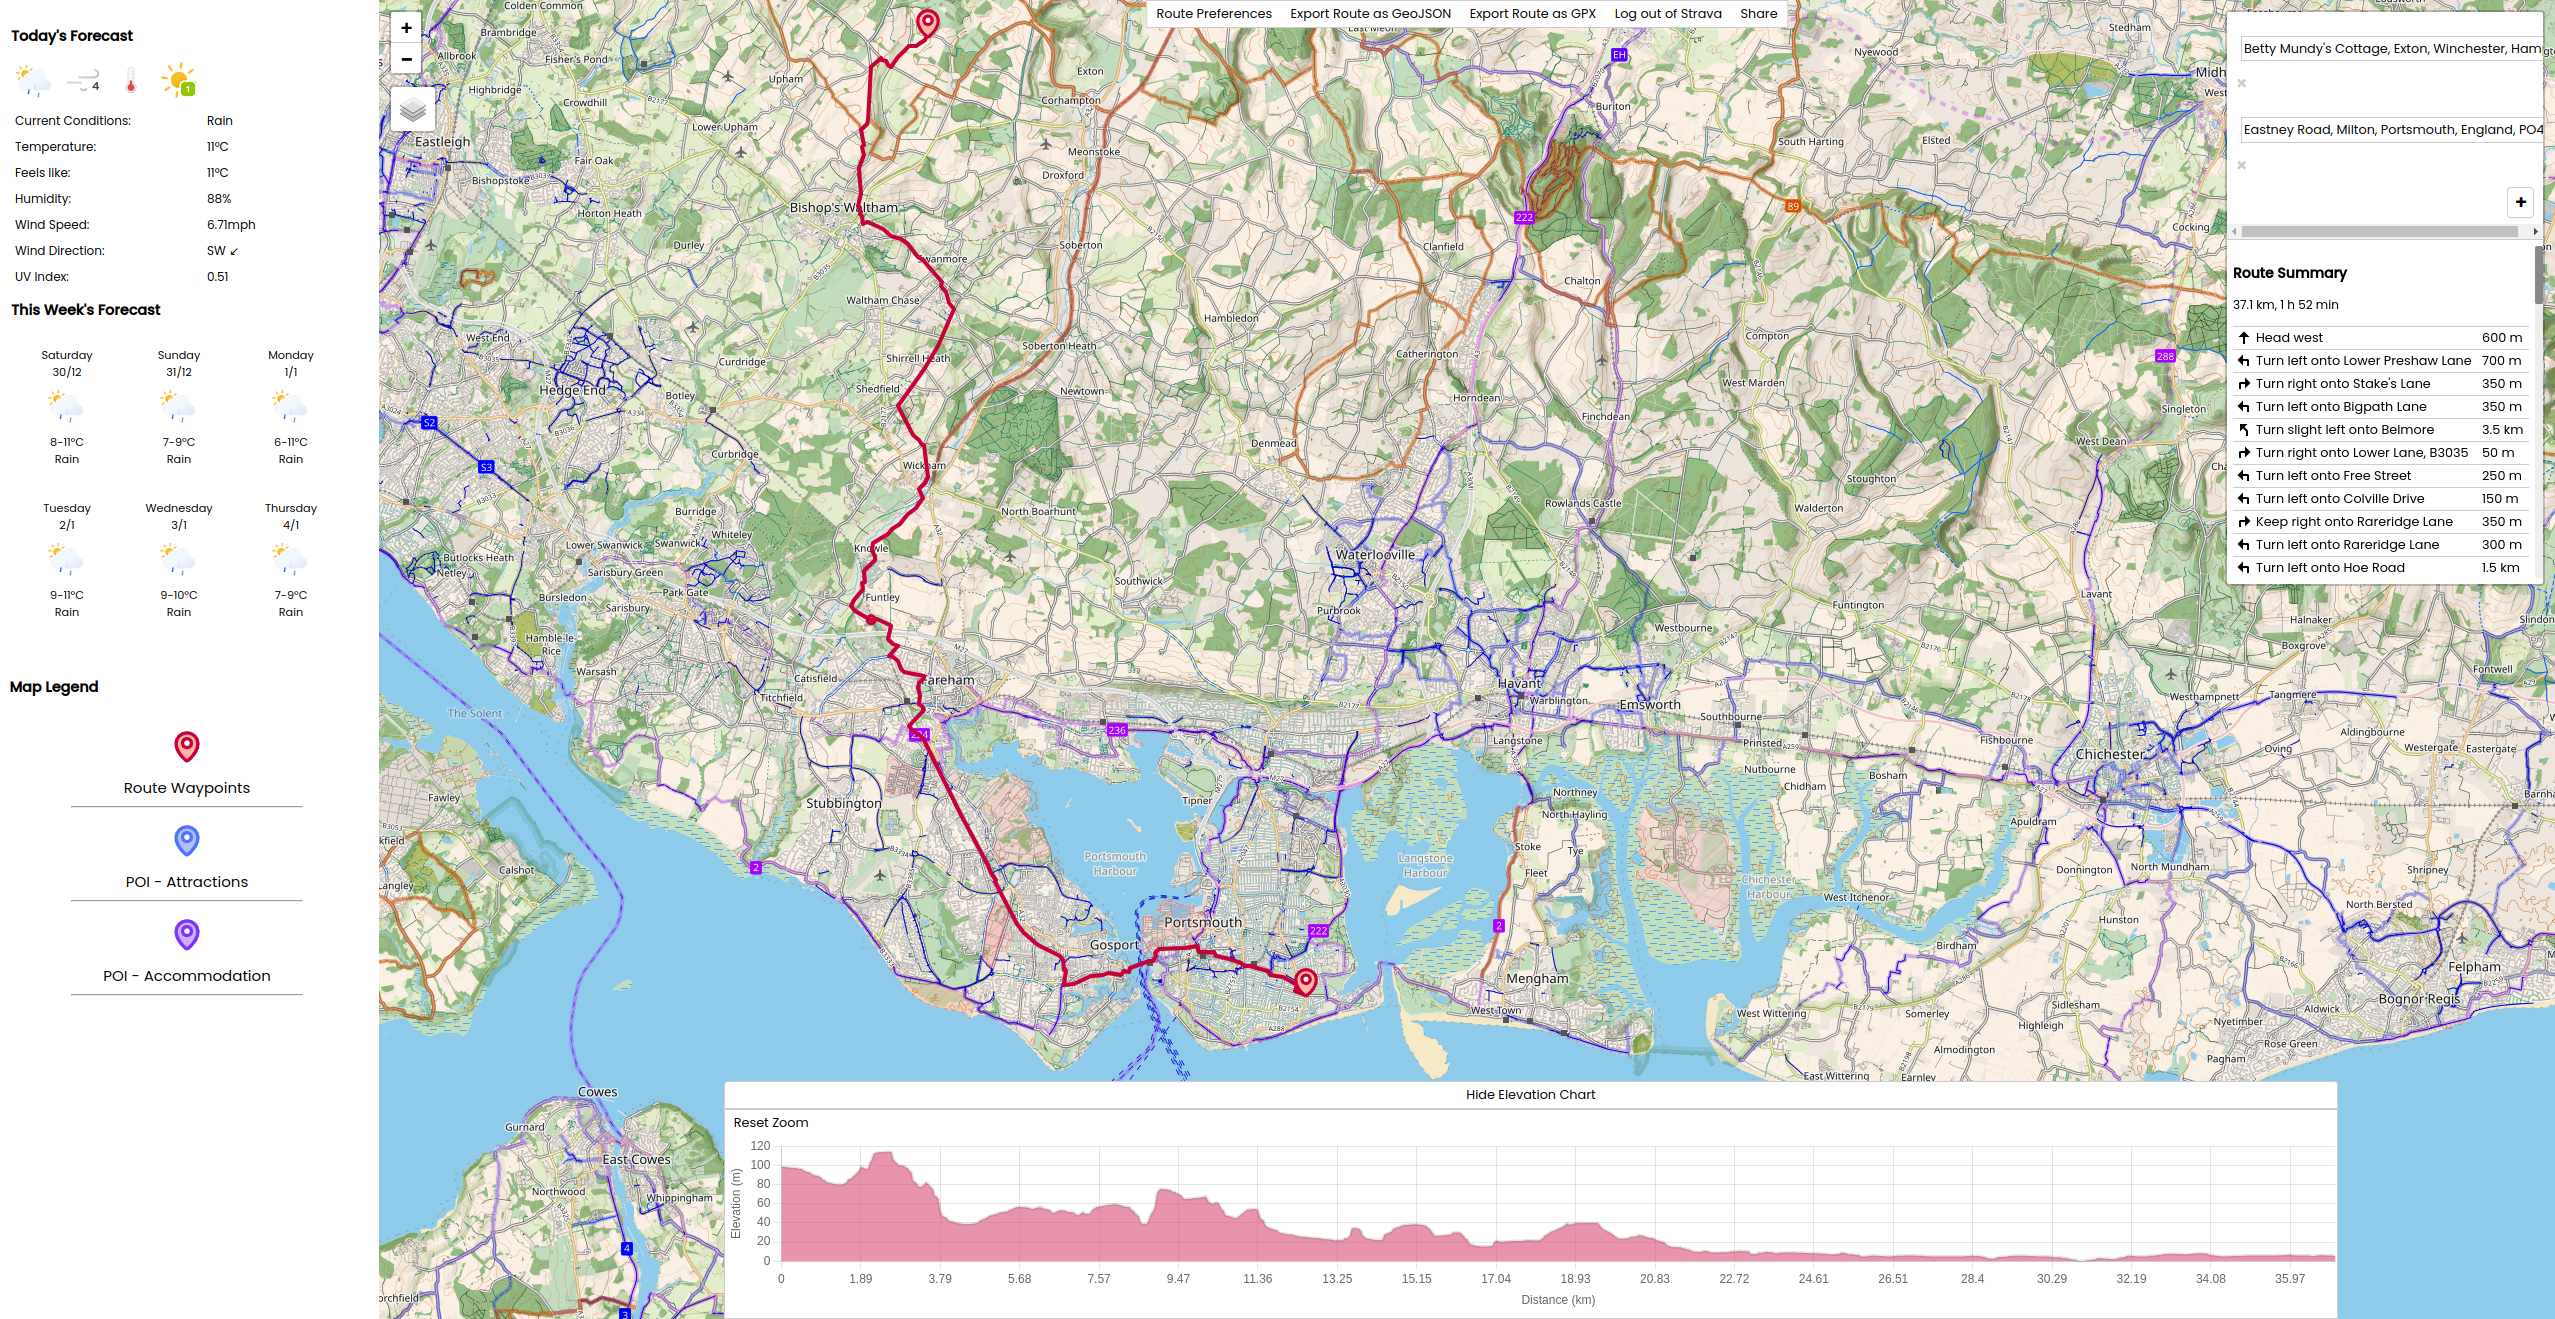
\includegraphics[width=425px]{figures/Progress Images/Iteration-2/SR30/SR30-Zoom Elevation Chart and Fly Map to same bounds.png}
    \caption{Chart Zoom and Map Pan}
    \label{fig:chart-zoom-map-pan}
\end{figure}

\begin{figure}[!ht]
    \centering
    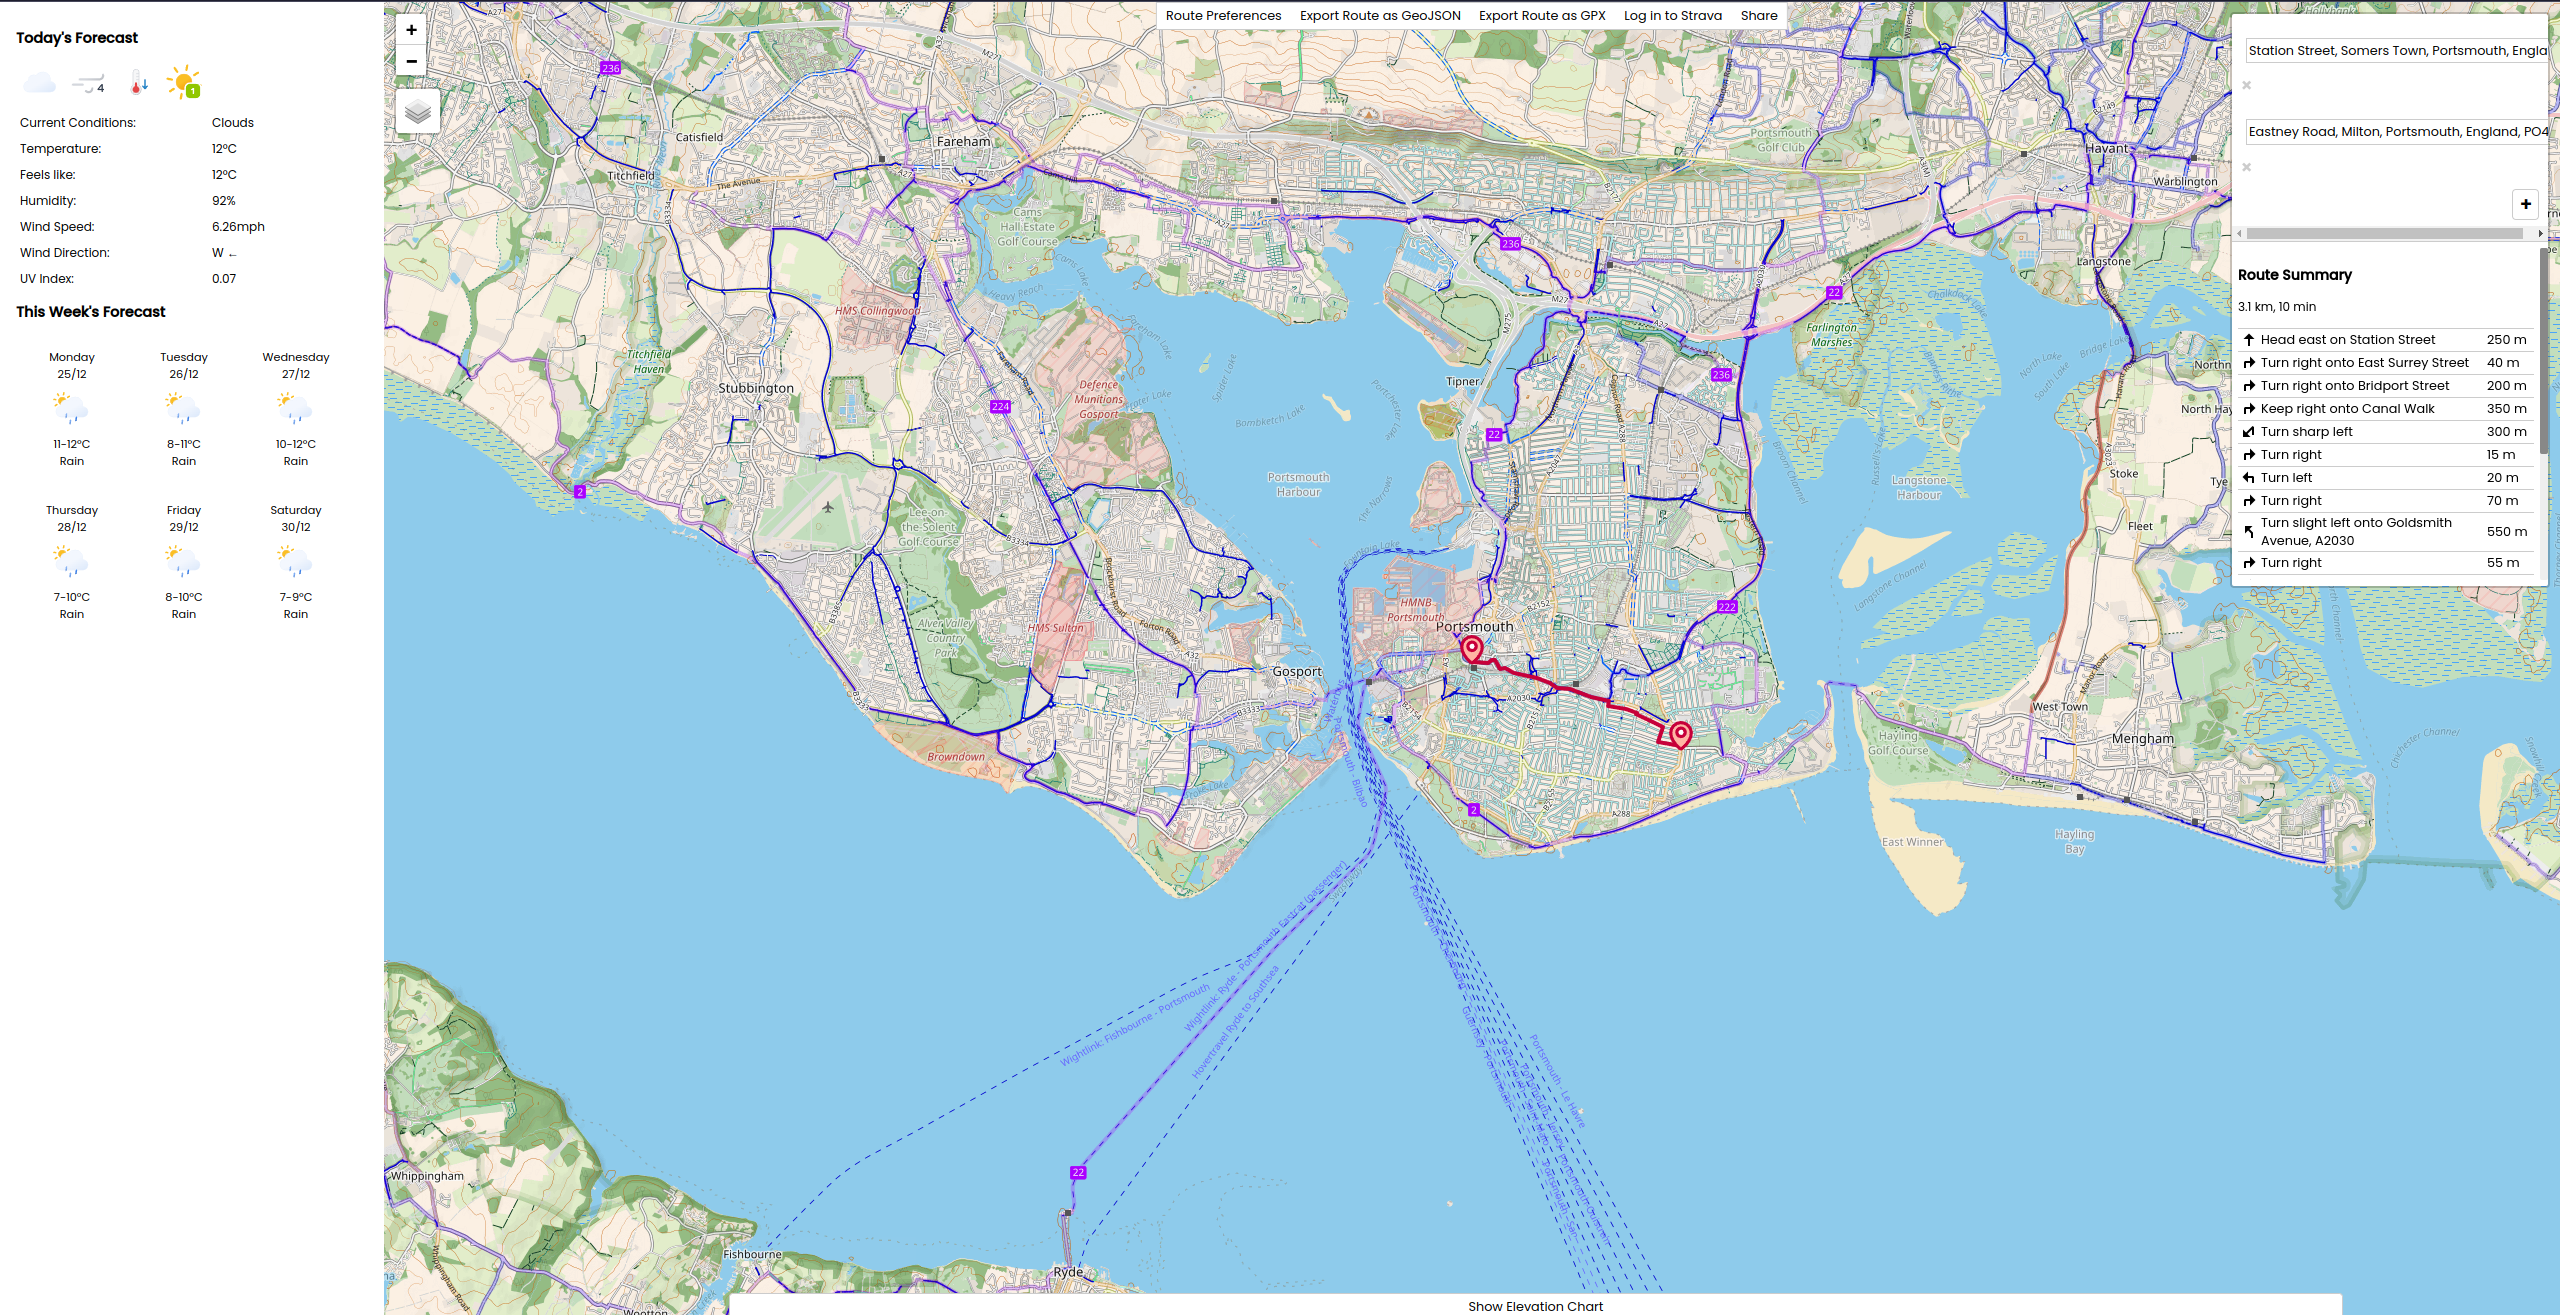
\includegraphics[width=425px]{figures/Progress Images/Iteration-2/SR31/SR31 Colours updated and new waypoints.png}
    \caption{Colour update, new waypoints}
    \label{fig:colours-waypoints}
\end{figure}

\begin{figure}[!ht]
    \centering
    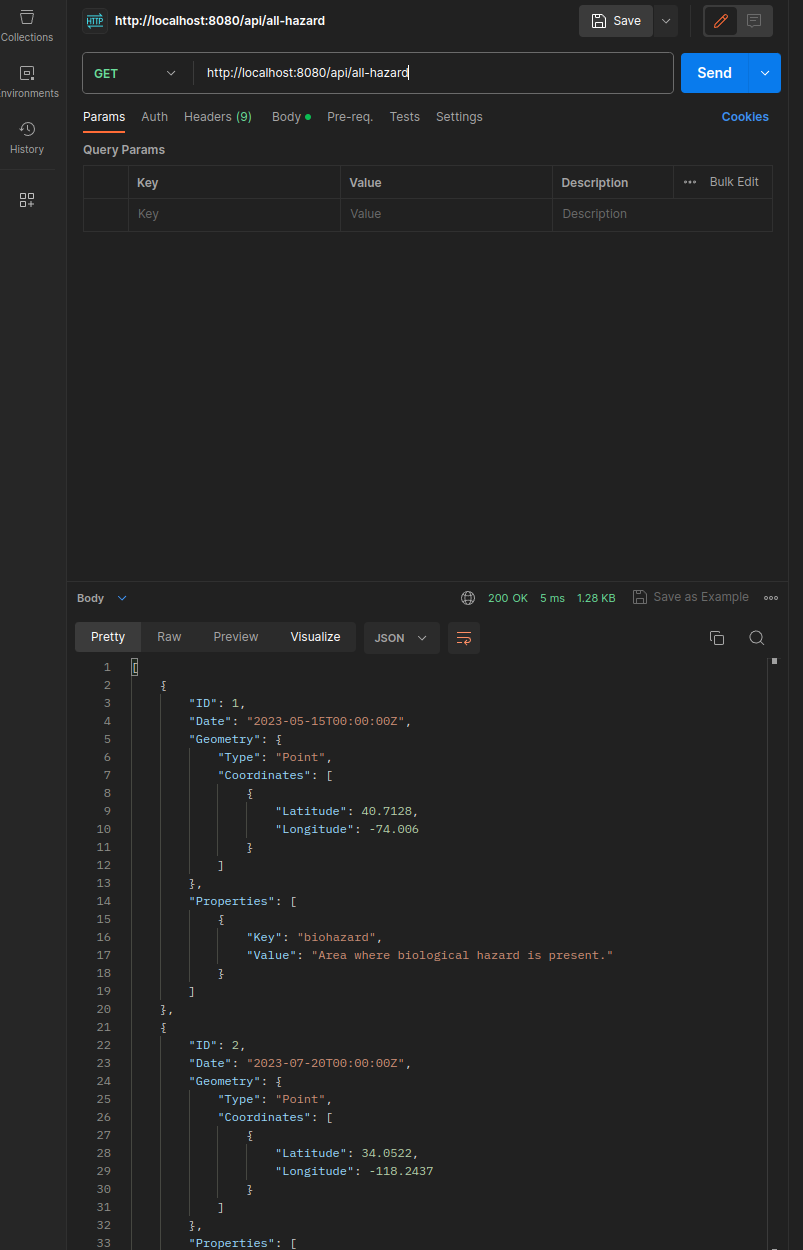
\includegraphics[width=425px]{figures/Progress Images/Iteration-2/SR32-37/SR32 - Basic API for selecting hazards.png}
    \caption{API for selecting hazards}
    \label{fig:select-hazard}
\end{figure}

\begin{figure}[!ht]
    \centering
    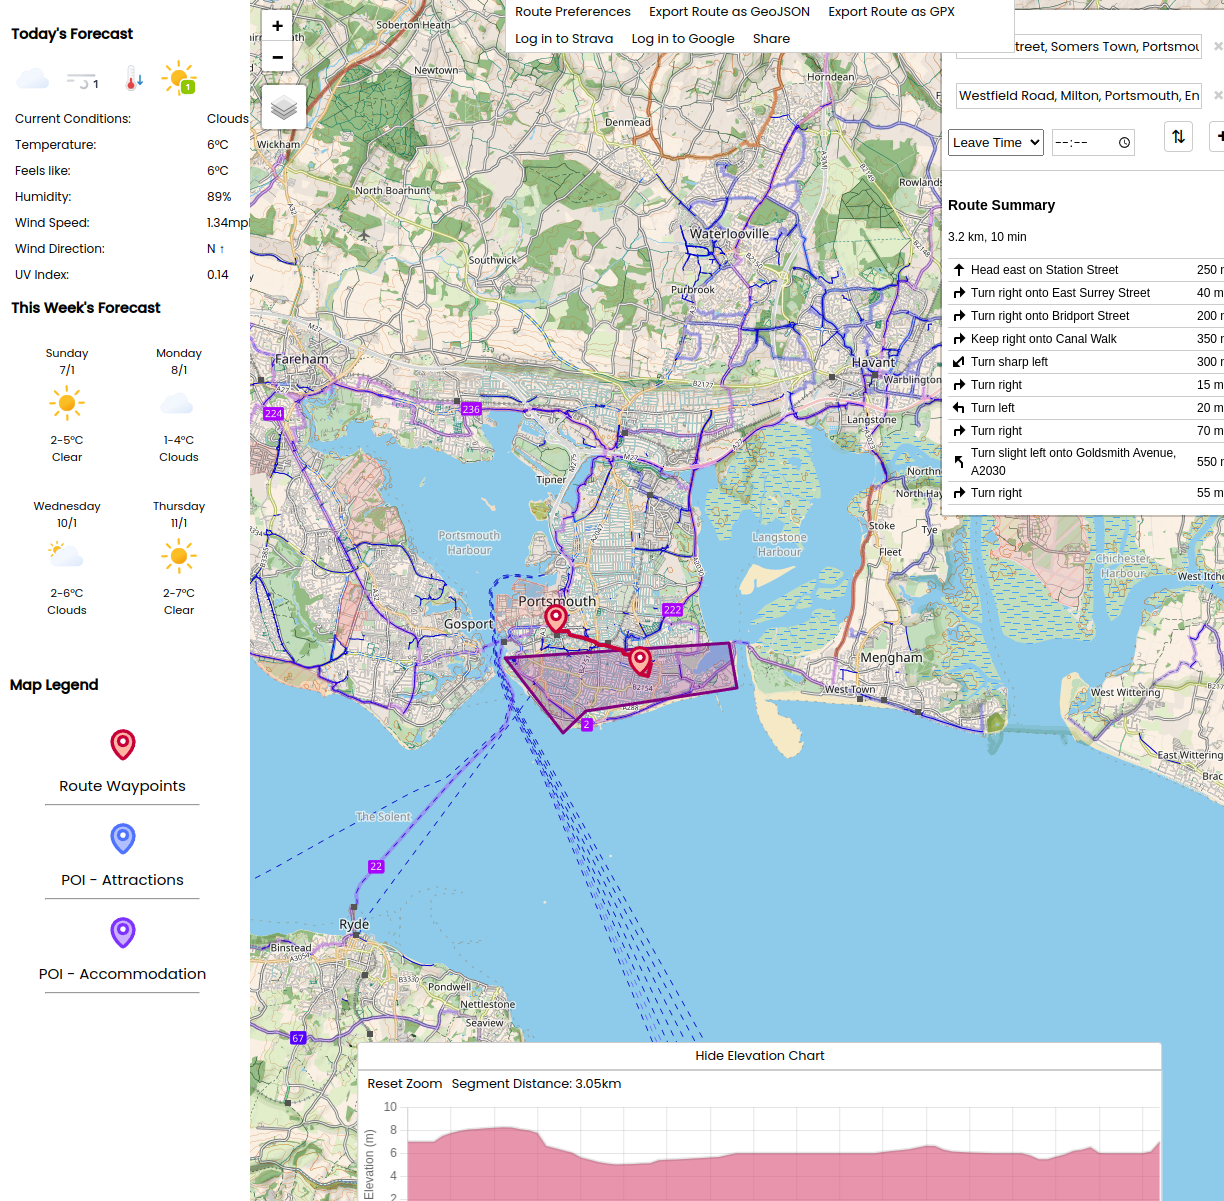
\includegraphics[width=425px]{figures/Progress Images/Iteration-2/SR32-37/SR32 - Basic Polygon from API.png}
    \caption{API Polygon}
    \label{fig:polygon}
\end{figure}

\begin{figure}[!ht]
    \centering
    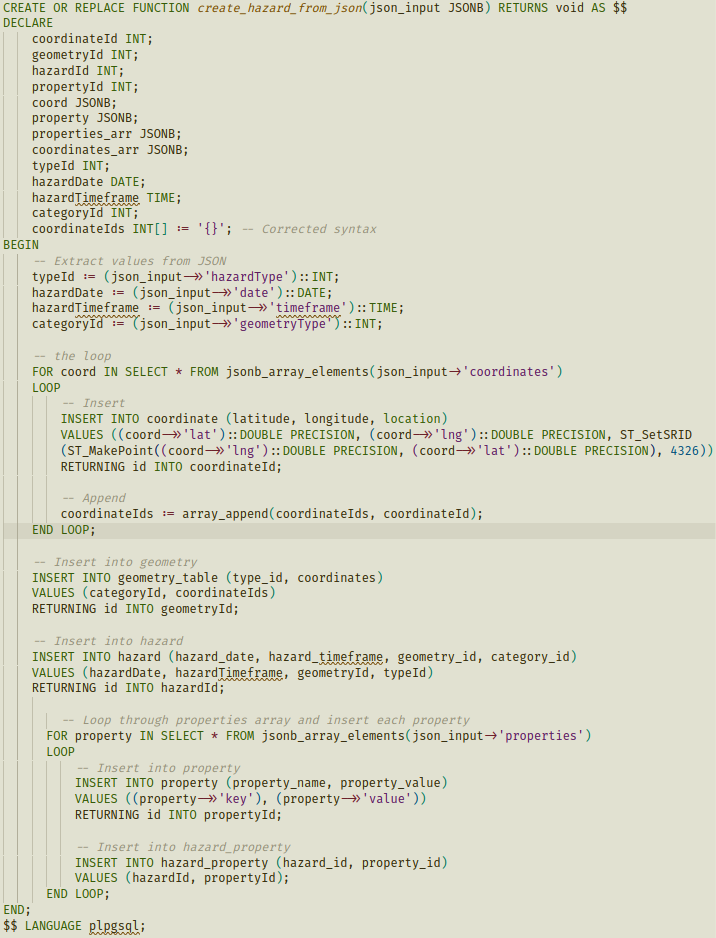
\includegraphics[width=425px]{figures/Progress Images/Iteration-2/SR32-37/sr32-add-hazard-point-sql.png}
    \caption{PLpgSQL Function for adding hazard points}
    \label{fig:plpgsql-func}
\end{figure}

\begin{figure}[!ht]
    \centering
    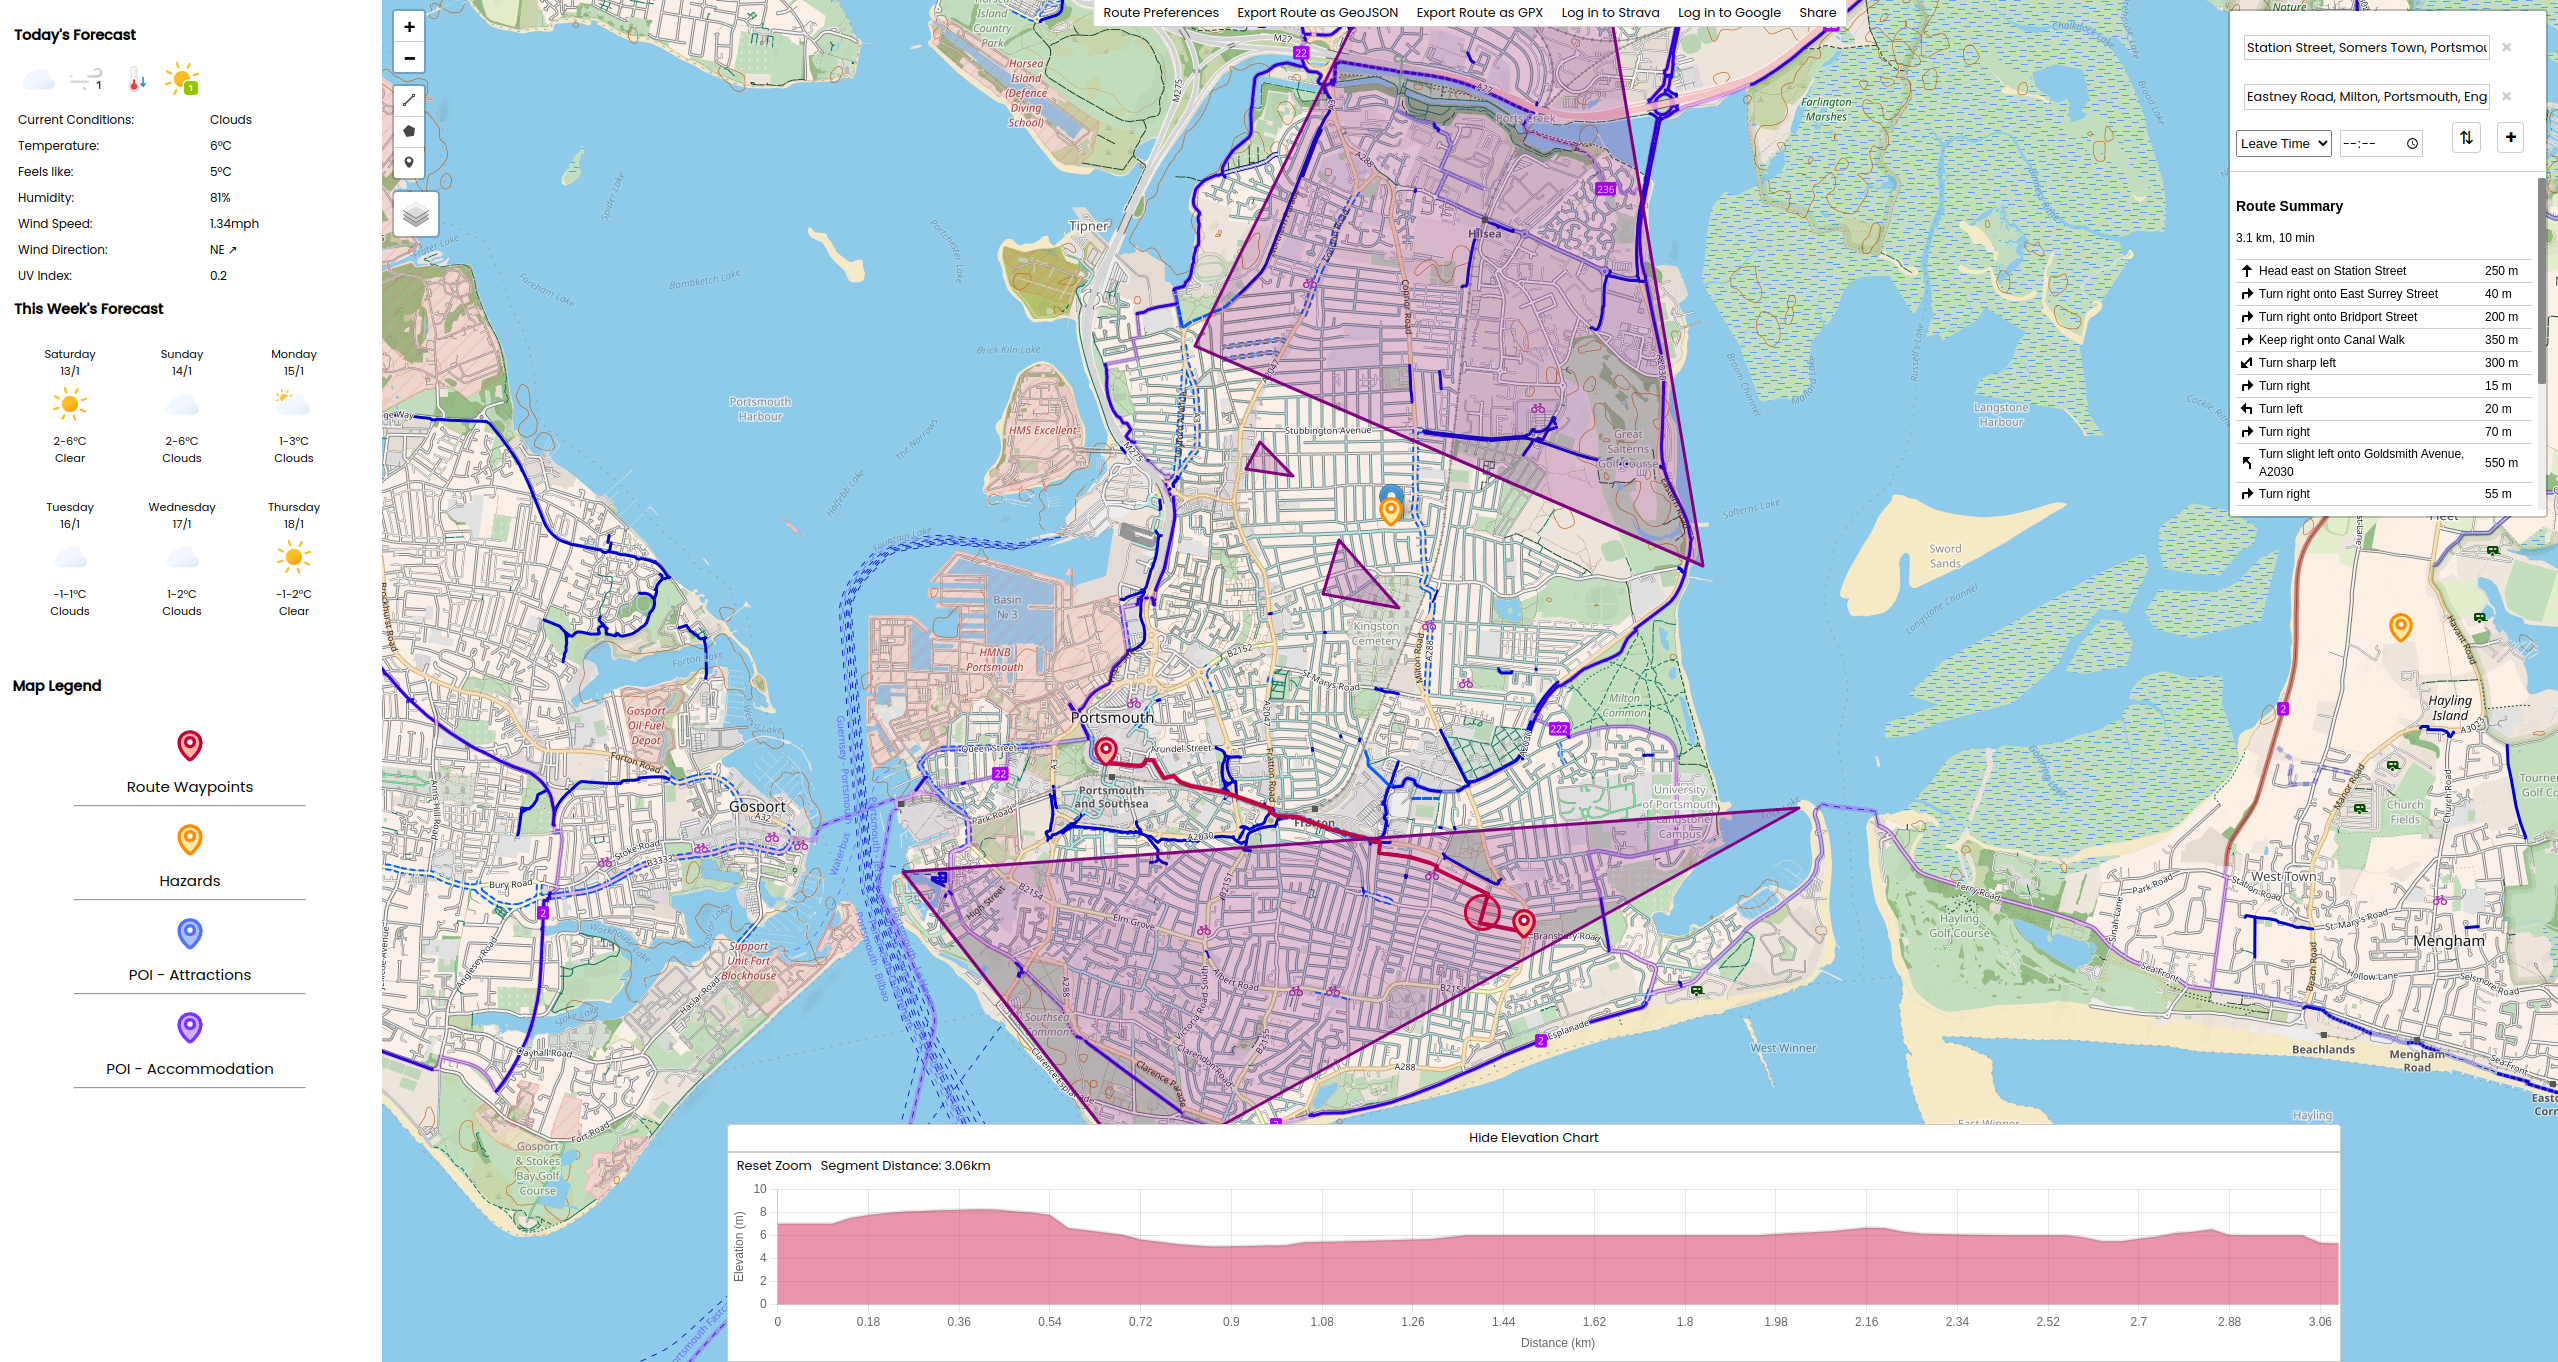
\includegraphics[width=425px]{figures/Progress Images/Iteration-2/SR32-37/sr32-add-polygon-marker-to-map.png}
    \caption{Add Polygon Marker to Map}
    \label{fig:add-polygon-marker}
\end{figure}

\begin{figure}[!ht]
    \centering
    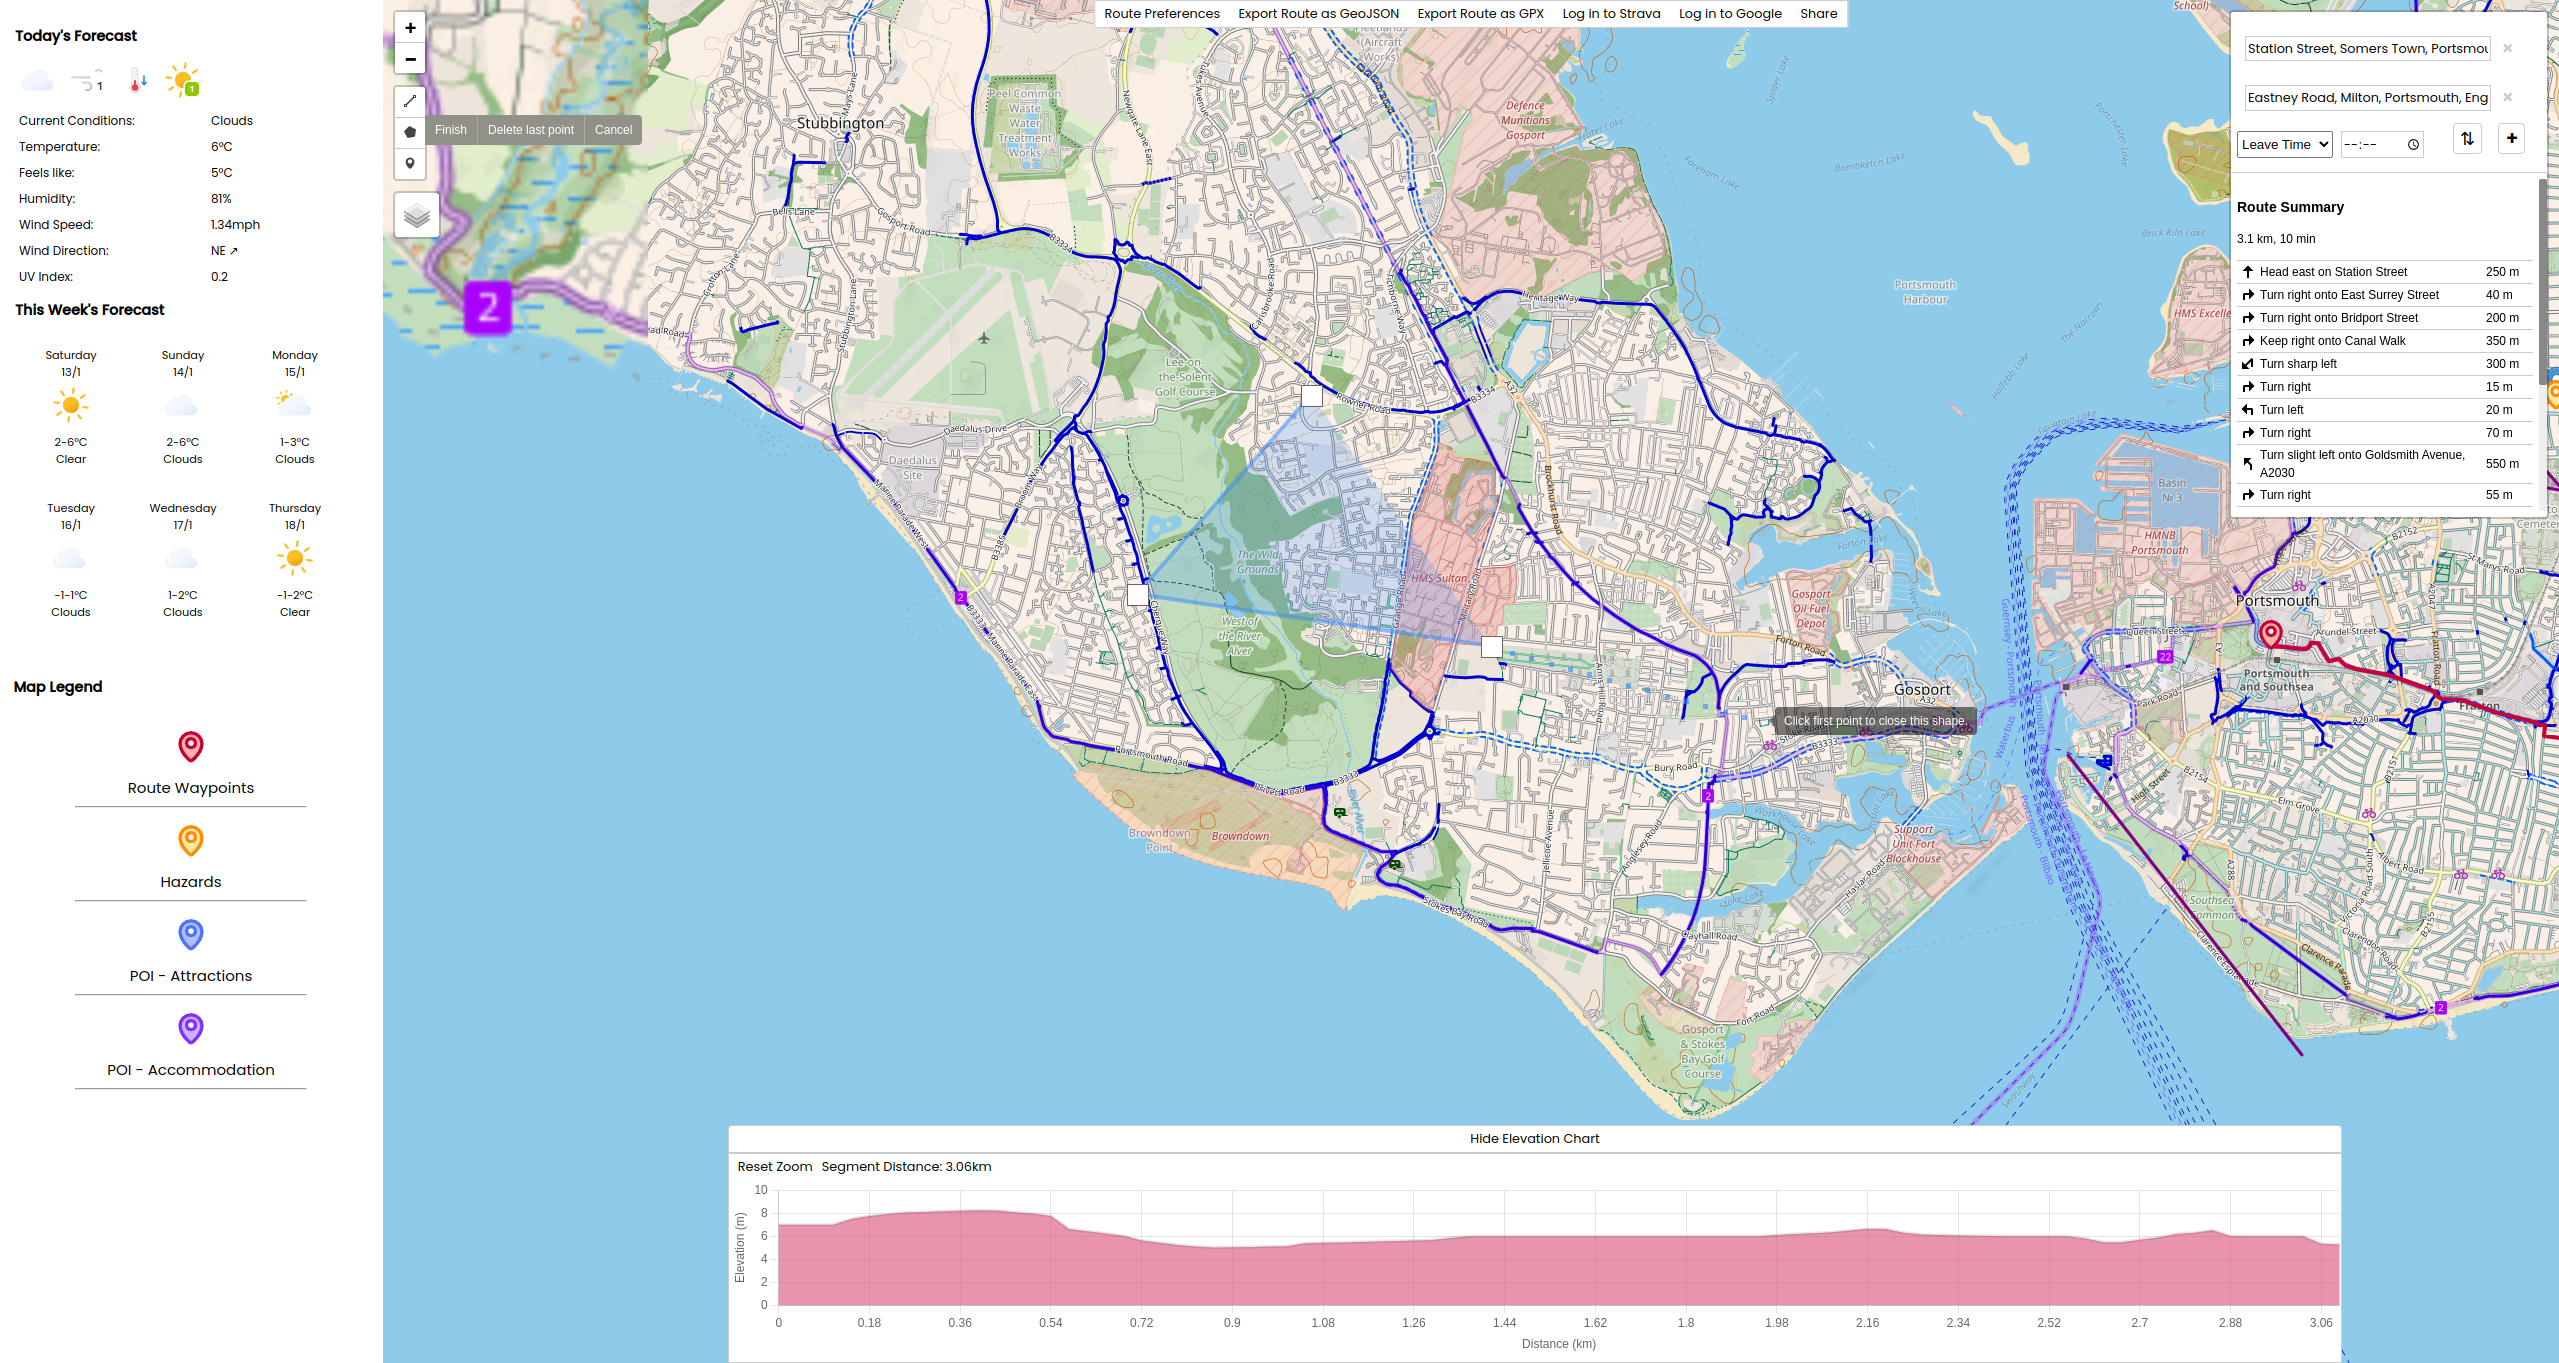
\includegraphics[width=425px]{figures/Progress Images/Iteration-2/SR32-37/sr32-create-polygon.png}
    \caption{Create Hazard Polygon}
    \label{fig:create-polygon}
\end{figure}

\begin{figure}[!ht]
    \centering
    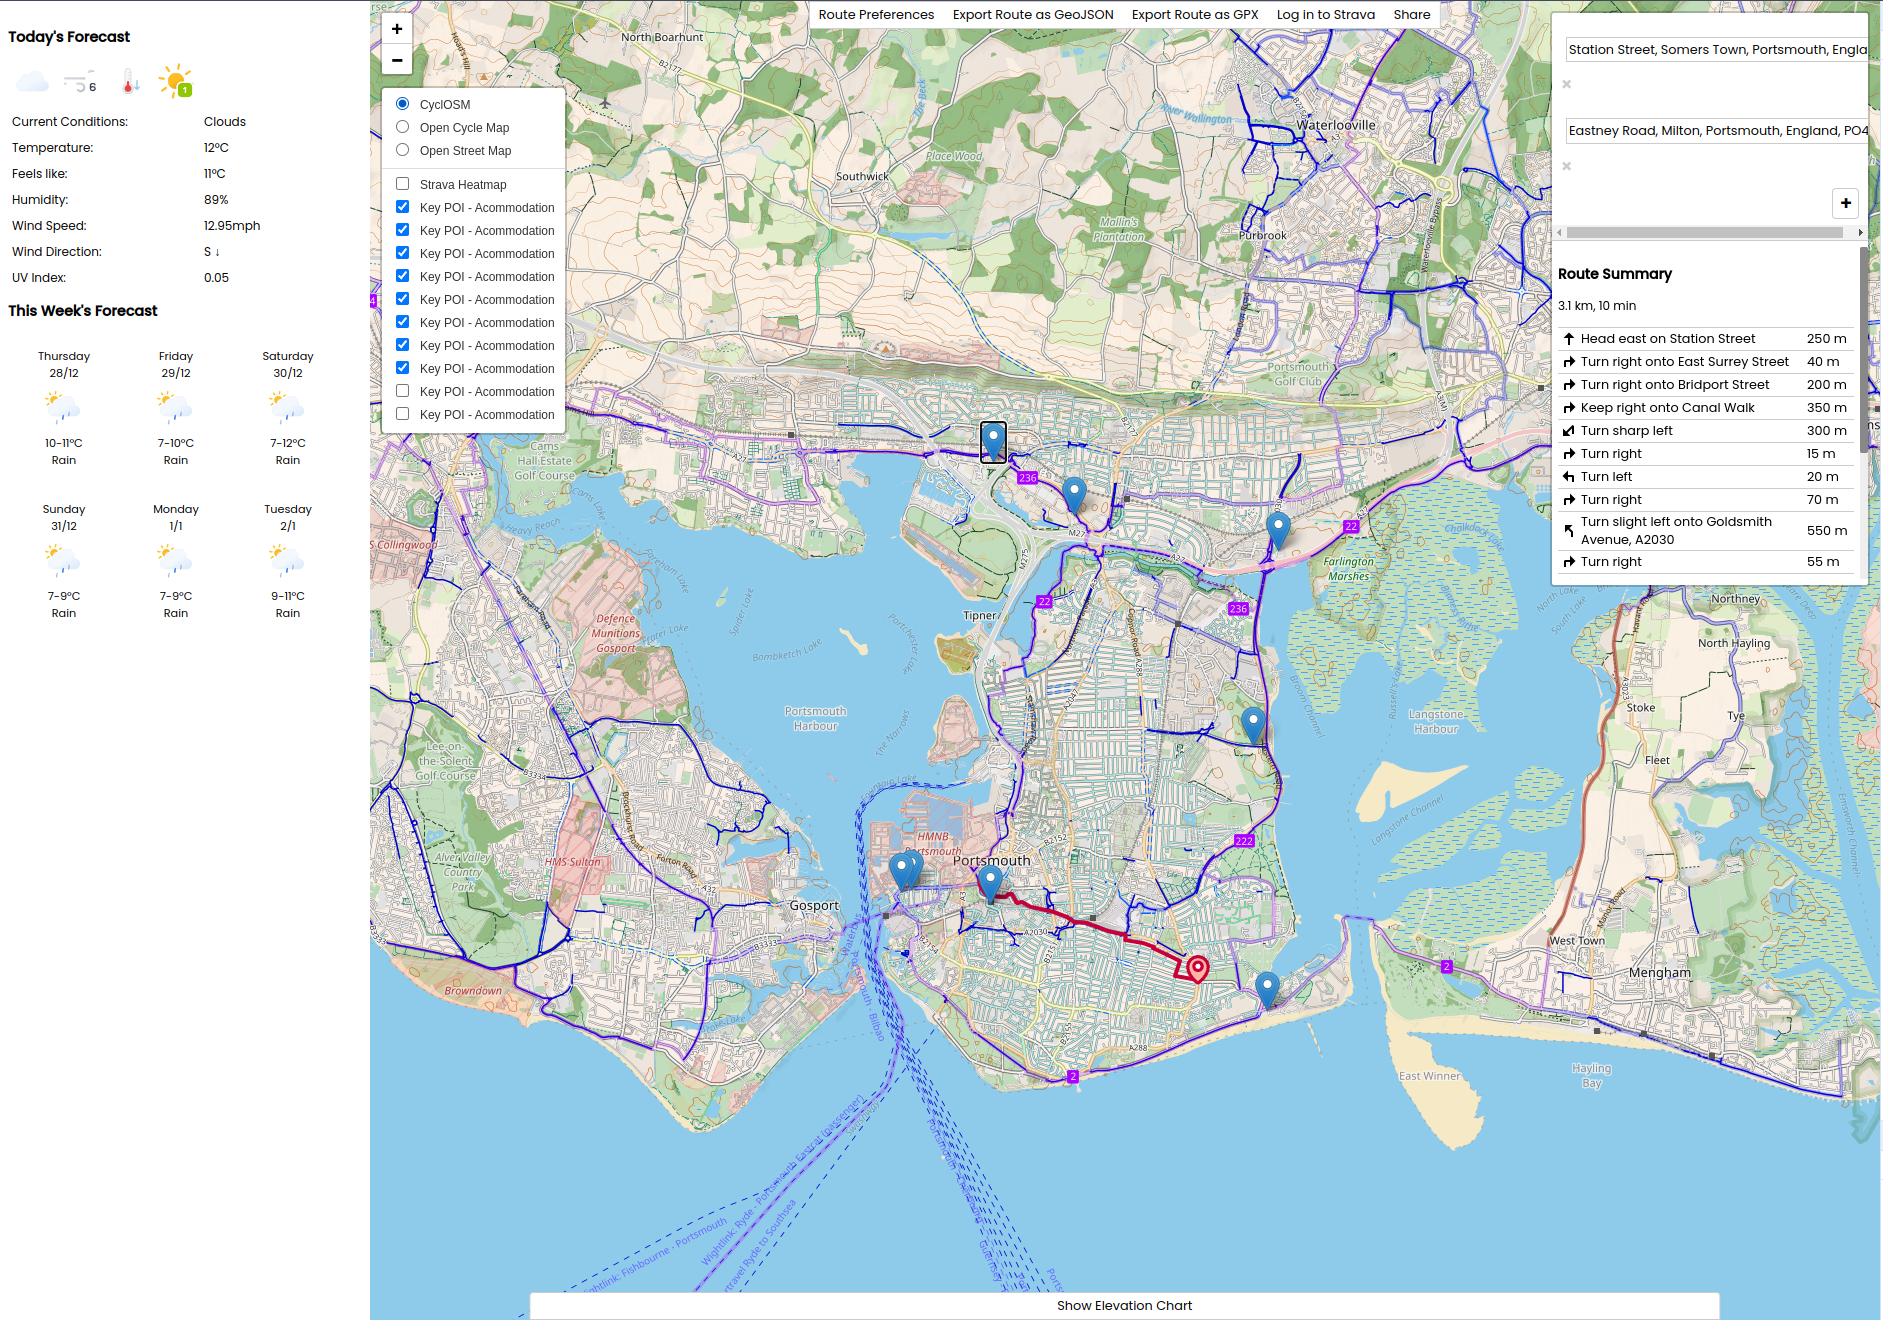
\includegraphics[width=425px]{figures/Progress Images/Iteration-2/SR40-45/SR40 - Issue, multiple layers .png}
    \caption{Issue creating map layers}
    \label{fig:layer-issue}
\end{figure}

\begin{figure}[!ht]
    \centering
    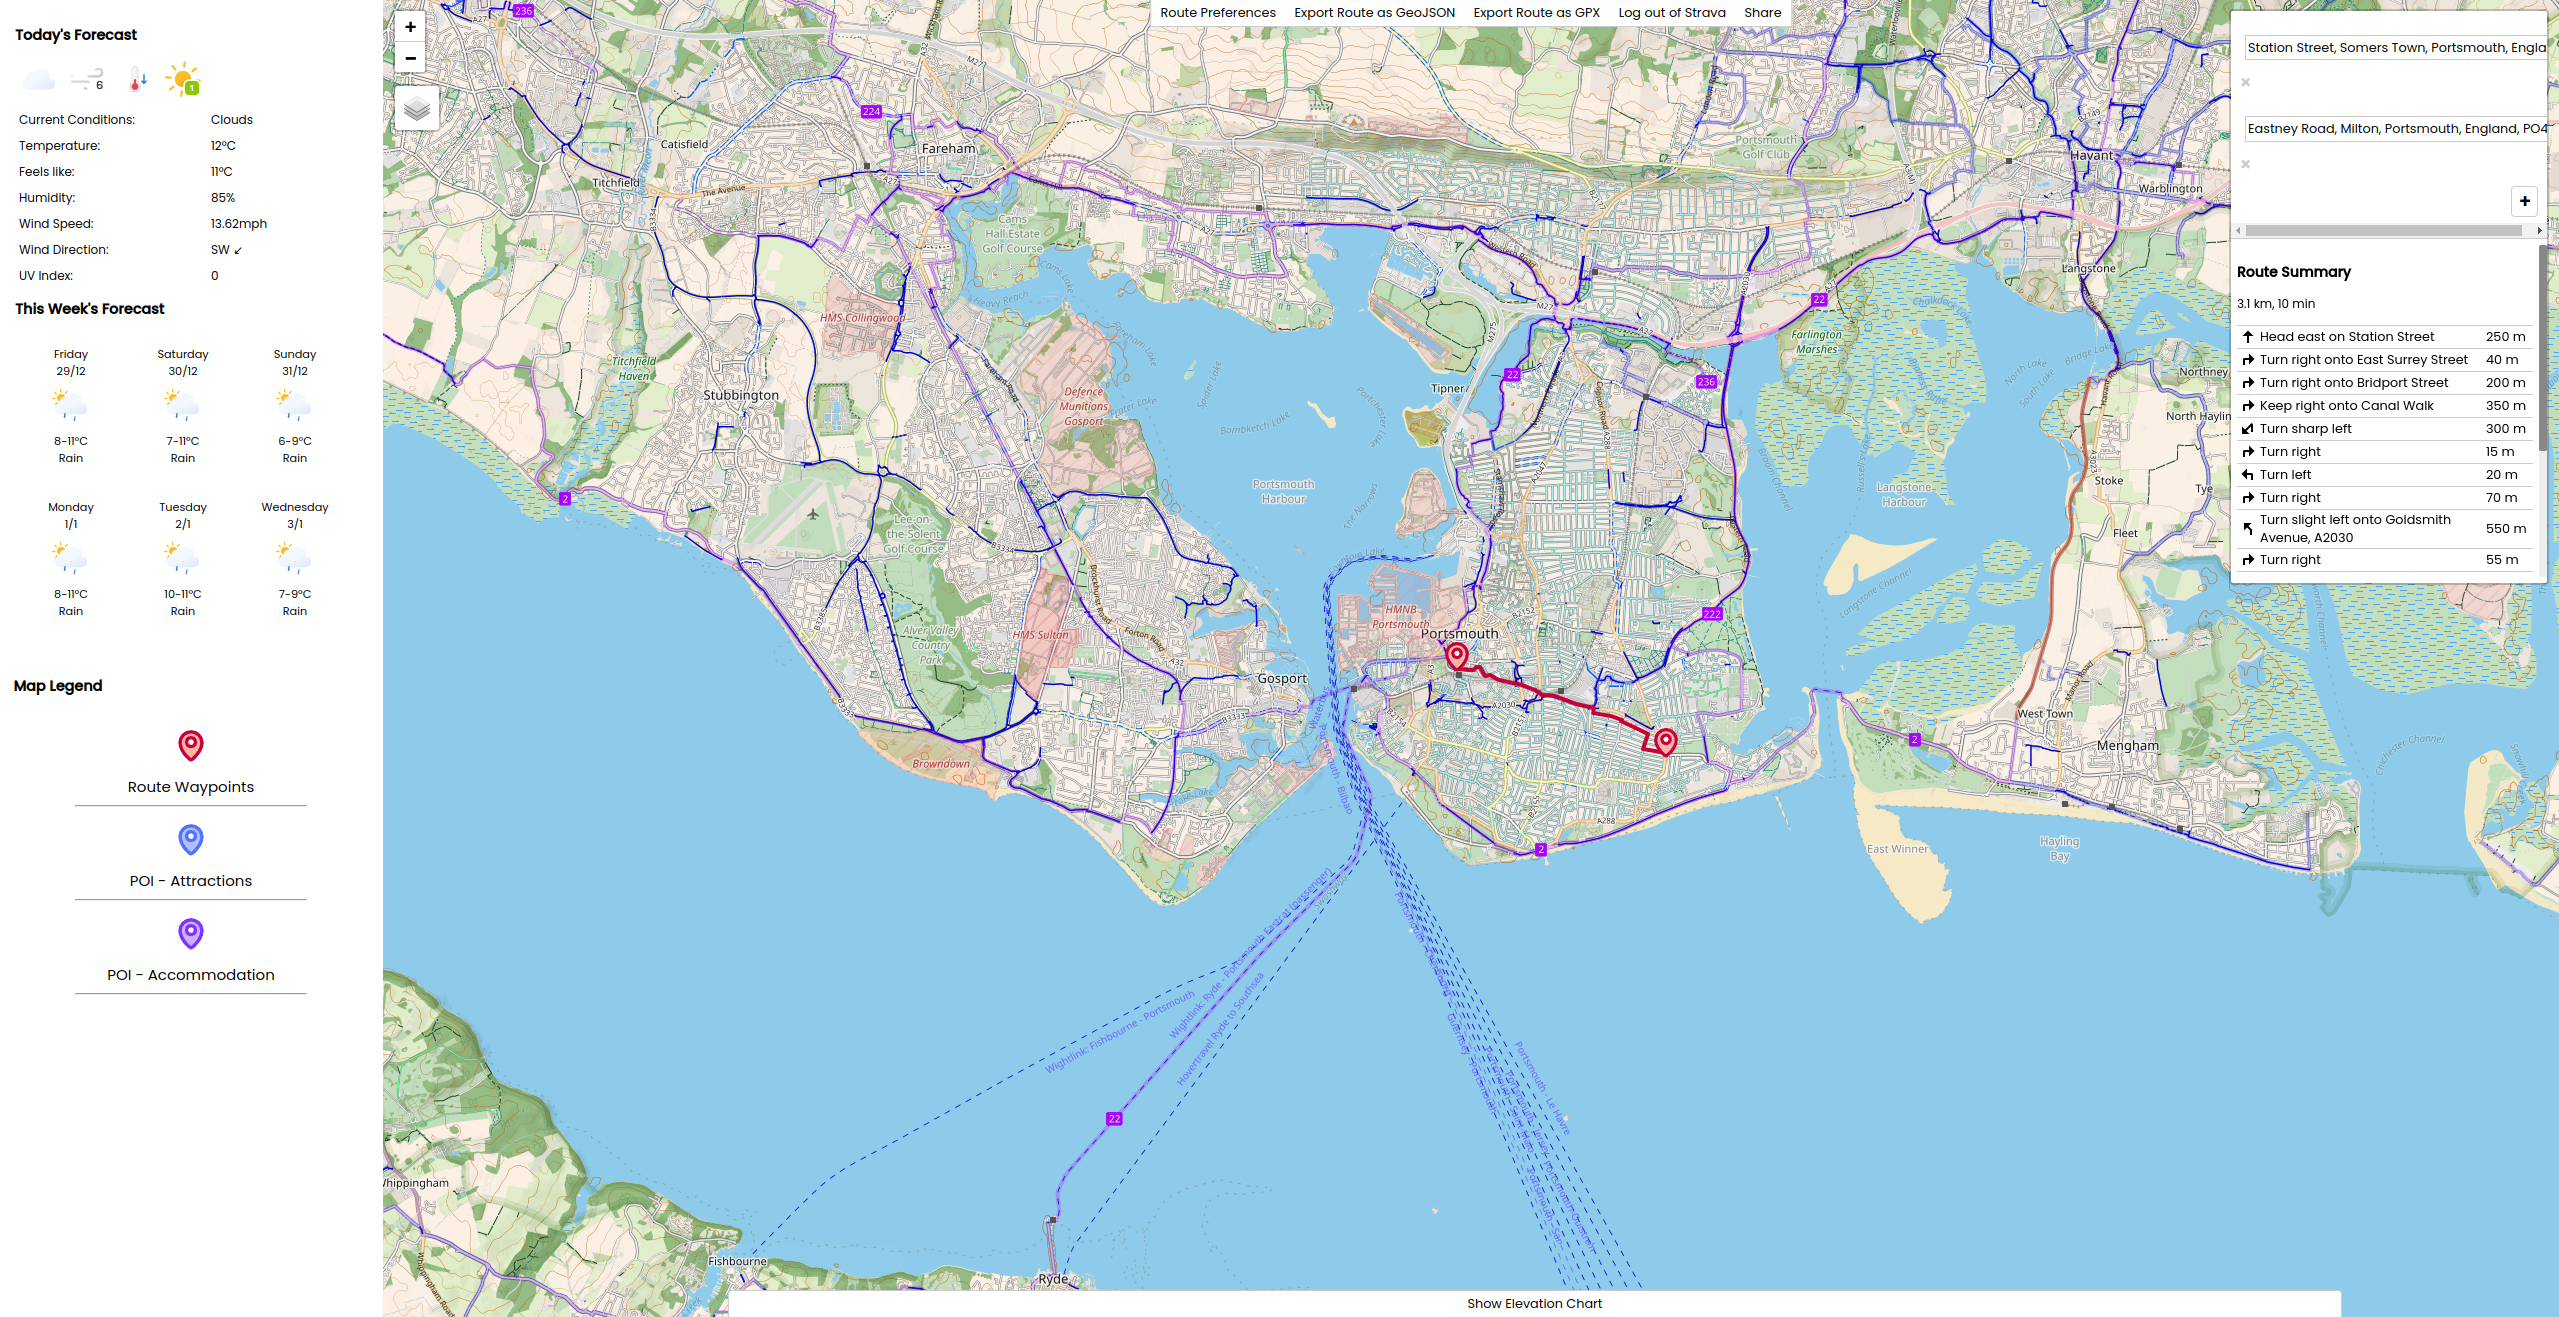
\includegraphics[width=425px]{figures/Progress Images/Iteration-2/SR40-45/SR40 - Map Legend.png}
    \caption{Map Legend}
    \label{fig:map-legend}
\end{figure}

\begin{figure}[!ht]
    \centering
    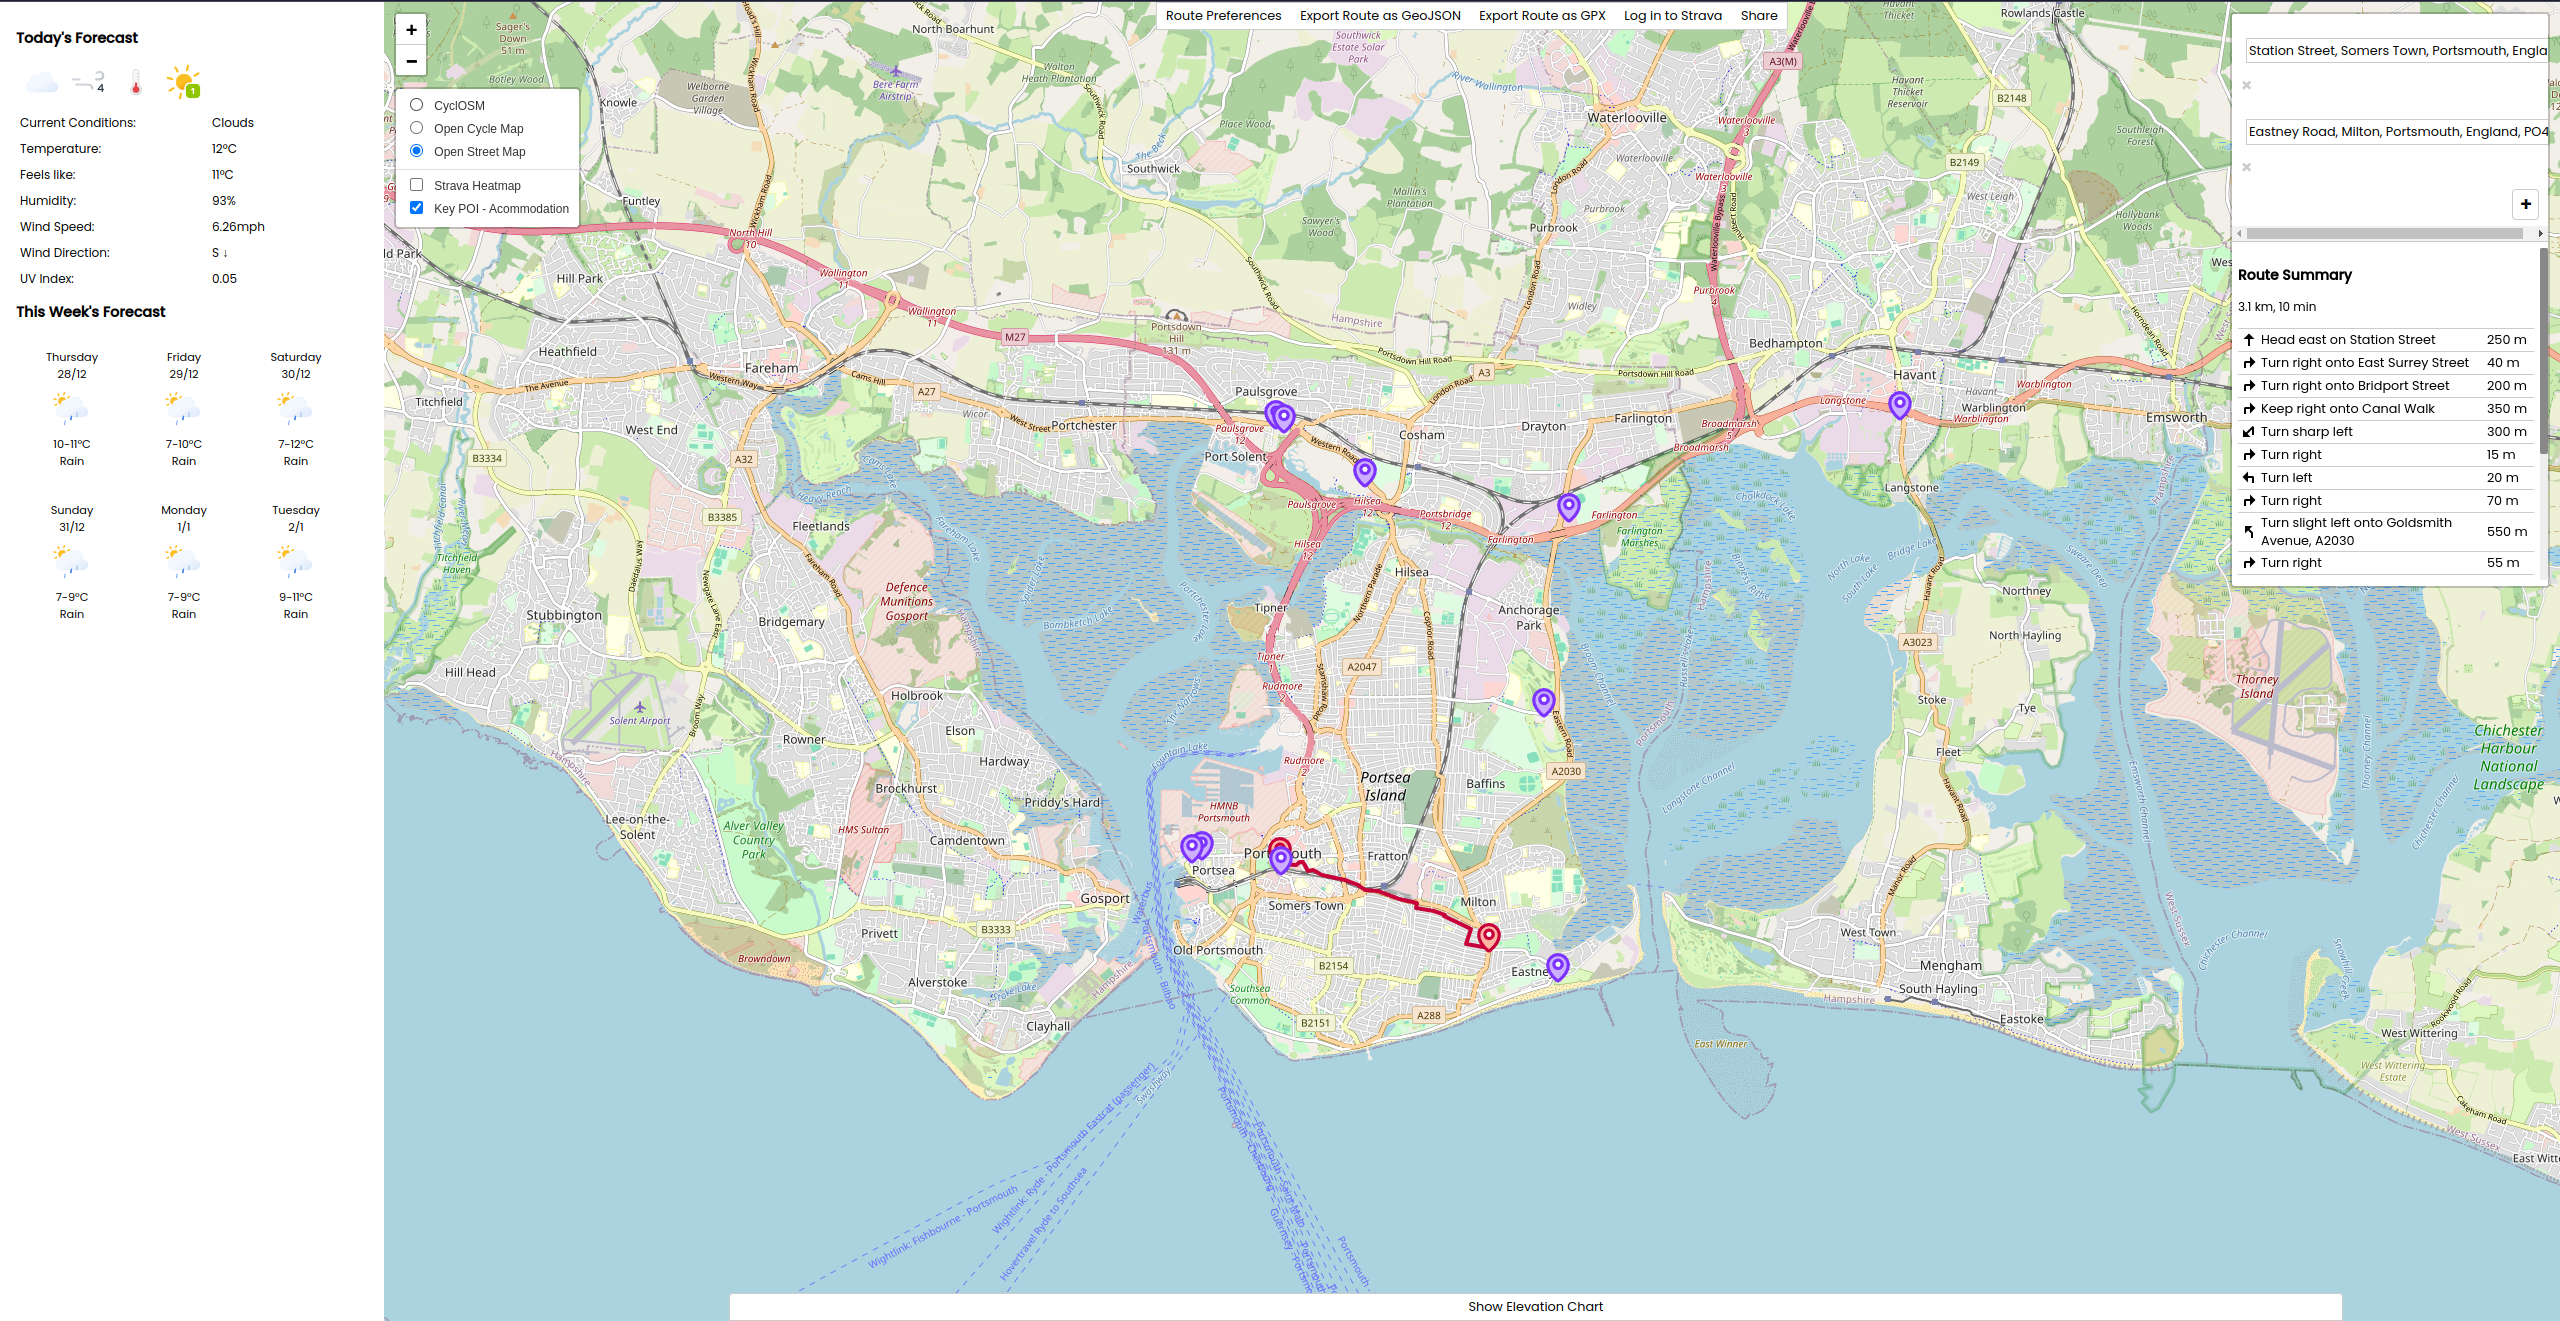
\includegraphics[width=425px]{figures/Progress Images/Iteration-2/SR40-45/SR41 - Accommodation KeyPOI.png}
    \caption{Accommodation KeyPOI Layer}
    \label{fig:accommodation-layer}
\end{figure}

\begin{figure}[!ht]
    \centering
    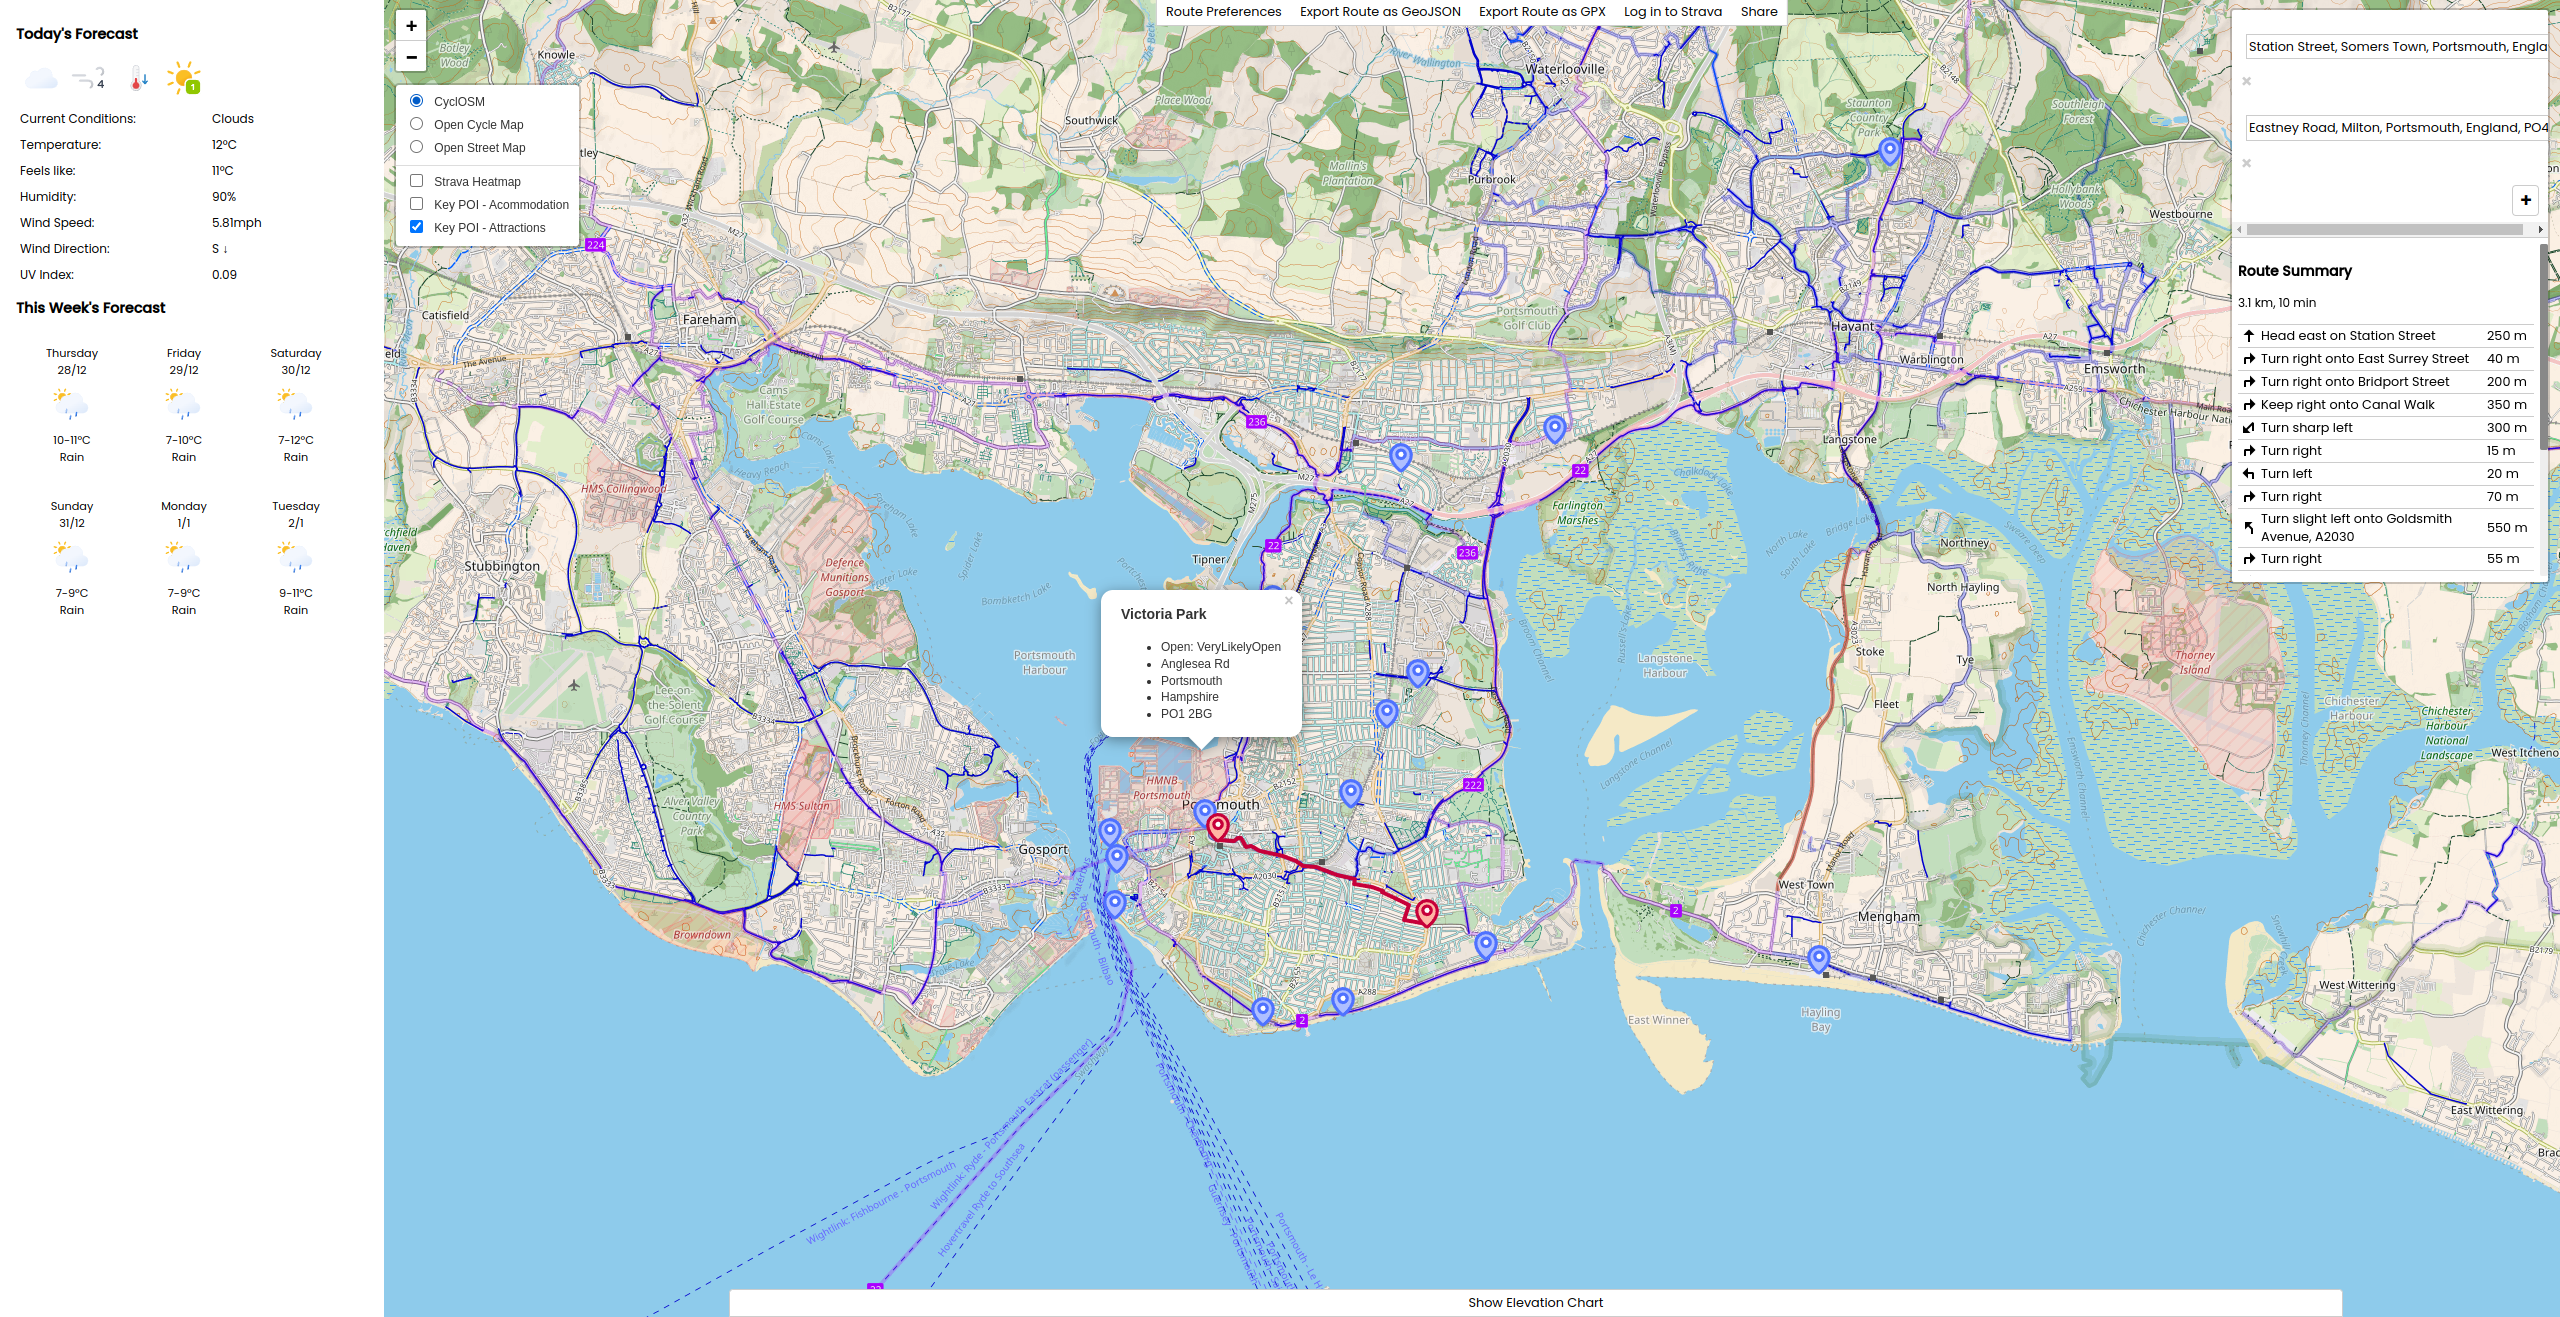
\includegraphics[width=425px]{figures/Progress Images/Iteration-2/SR40-45/SR42 - Attractions KeyPOI.png}
    \caption{Attractions KeyPOI Layer}
    \label{fig:attractions-layer}
\end{figure}
